\documentclass[a4paper,authoryear,review]{elsarticle}

\usepackage[utf8]{inputenc}
\usepackage{amssymb}
\usepackage{lineno}
\usepackage{url}
\usepackage{hyperref}
\usepackage{caption}
\usepackage{subcaption}
\usepackage{graphicx}
\usepackage{adjustbox}
\usepackage{epstopdf}
\usepackage{gensymb}
\usepackage{xcolor,colortbl}
% \usepackage[table,xcdraw]{xcolor}
% If you use beamer only pass "xcolor=table" option, i.e. \documentclass[xcolor=table]{beamer}
\usepackage[normalem]{ulem}
\useunder{\uline}{\ul}{}
%TODO: remover
\DeclareUnicodeCharacter{0301}{\'{e}}
\hypersetup{unicode=true,
           colorlinks=true,
           linkcolor=blue,
           citecolor=blue,
           filecolor=red,
           urlcolor=blue,
           breaklinks=true
           }

\journal{Journal of Computers and Electronics in Agriculture}

%% `Elsevier LaTeX' style
\bibliographystyle{elsarticle-harv}
%%%%%%%%%%%%%%%%%%%%%%%

\begin{document}

\begin{frontmatter}

\title{Localización 2D de yemas de vid utilizando técnicas de deep learning}

\author[utn,uncuyo]{Diego Sebastián Pérez\corref{cor1}}
\ead{sebastian.perez@frm.utn.edu.ar}

\author[utn]{Wenceslao Villegas}
\ead{villegaswences@gmail.com}

\author[utn]{Carlos Ariel Diaz}
\ead{carlos.diaz@frm.utn.edu.ar}

\author[conicet]{Facundo Bromberg}
\ead{fbromberg@frm.utn.edu.ar}

\address[utn]{Universidad Tecnológica Nacional, Facultad Regional Mendoza, Laboratorio de Inteligencia Artificial DHARMa, Dpto. de Sistemas de la Información. Rodríguez 273, CP 5500, Mendoza, Argentina.}

\address[uncuyo]{Universidad Nacional de Cuyo, Instituto universitario para las Tecnologías de la Información y las Comunicaciones, CONICET. Padre Jorge Contreras 1300, CP 5500, Mendoza, Argentina.}

\address[conicet]{Universidad Tecnológica Nacional, Facultad Regional Mendoza, CONICET, Laboratorio de Inteligencia Artificial DHARMa, Dpto. de Sistemas de la Información. Rodríguez 273, CP 5500, Mendoza, Argentina.}

\cortext[cor1]{Corresponding author}

\begin{abstract}
TODO
\end{abstract}

\begin{keyword}
Computer vision \sep Fully Convolutional Network \sep Grapevine bud localization \sep Scanning-window detection \sep Precision viticulture
\end{keyword}

\end{frontmatter}

\linenumbers

%#######################################################################
%#######################################################################
\section{Introduction} 

% Problem: detection, Solution: FCN
In this work we propose a solution for the autonomous detection of grapevine buds within 2D images of vineyards captured in natural field conditions. Our proposed approach is based on \emph{Fully Convolutional Networks} (\textbf{FCN}) \citep{long2015fully, shelhamer2017fully}, a kind of deep learning model specific for computer vision applications. Our solution adds in the historical quest for more and better quality information about different vineyard processes that impact on the productivity of grapevines and quality of their grapes. 

% ¿why bud related variables are important?  fertility
% ¿why fertility is important? main goal of grapevine producers is to estimate and the guarantee the grapevine production.
%
For centuries agronomists have been producing models of the most relevant plant processes (i.e. fruit quality and yield, soil profiling, vine health),  and vineyard managers have been recollecting a diverse corpus of information for feeding these models.  Better and more efficient measuring procedures resulted in more information with its corresponding impact on the quality of models’ outcomes, while inspiring researchers to push the boundaries for producing more sophisticated models. Such information consists of a large set of variables for assessing different aspects of the parts of the plant involved in these processes: trunks, leaves, berries, buds, shoots, flowers, bunches, canes. 
%
Nowadays technology is pushing once again the possibilities in the quality and throughput of these measurements, with digital and autonomous measurement procedures that improve over manual measurement procedures. The discipline is experiencing a transition, with many of its variables, e.g.,  
Variables such as conteo de yemas no brotadas, número de flores, cantidad de bayas, cantidad de racimos, número de plantas por claro, riqueza de poda, brotes totales, brotes de yemas francas, diámetro del tronco, longitud de entrenudos, longitud de 1er alambre descubierto y longitud del brote, entre tantos otros  \citep{pellegrino2005towards, intrigliolo2007evaluation, reynolds2009influence}, \citep{matese2015technology, ozdemir2017precision, poni2018grapevine} are still being measured manually through visual inspection, resulting in large labor costs that limits the measurement campaigns to only small samples of data, that even with the use of statistical inference or spatial interpolation techniques impose a bound in the quality of the outcomes \citep{whelan1996spatial, borgogno2018comparison, taylor2019considerations}. 
%
In some cases this is exacerbated by the need of experts for a proper measurement, such as the case of variables associated to the phenological state of the plant such as hinchado de yema, apertura de yema, inflorescencia, floración, envero, maduración, entre otras \citep{lorenz1995growth, zapata2017predicting}; or by measurement procedure that requires the destruction of the part of the plant being measured, preventing any tracking of the variables overtime. Such is the case for the measurement of leaves área, el peso del racimo, el peso de las bayas o el peso de poda \citep{kliewer2005leaf, diago2012grapevine, liu2013towards}. 
%
%

%
Precision viticulture in general \citep{bramley2004understanding, matese2015technology, ozdemir2017precision}, and computer vision algorithms \cite{seng2018computer} in particular, has been growing in the last couple of decades, mainly for their potential for mitigating these limitations. These algorithms come along a promise of an unprecedented boost in the production of vineyard information, with much expectations not only on possible improvements in the quality of the models’ outcomes, but   in its potential to produce better models by feeding all this information to big data algorithms. 

%
In this work we contributed to this general endeavour with an algorithm for measuring variables related to one specific part of the plant: the bud; an organ of major importance for being the  grow point of the fruits, containing within all the productive potential of the plant \citep{may2000bud, vasconcelos2009flowering, keller2020science}. Our contribution of  autonomous bud detection not only enables the autonomous measurement of all bud related variables currently measured by agronomists (see Table 1 for a non-exhaustive list of bud related variables); but has the potential to enable the measurement of novel, yet important variable  that are currently impossible to be measured manually. One example is the total sunlight captured by the buds, that depends on the manually unfeasible task of determining the exact location of buds in 3D space.  Although the present work focuses on 2D detection, it could be easily upgraded to 3D by, for instance, integrating the 2D detection in the workflow proposed by \cite{diaz2018grapevine} (c.f. Section~\ref{sec:related} for some more details on this workflow).

%
Table \ref{tab:Tabla1} shows a non-exhaustive list of the most important bud related variables currently measured by vineyard managers [REF], accompanied by an assessment of the extent to which detection contributes in their measurement. The right-most column indicates what information beyond detection  is necessary to complete the measurement, while the middle columns labeled (i), (ii), and (iii) indicates the details of what specific aspects of the detection is required for that variable, whether it requires a good  \emph{segmentation}, i.e., the discrimination of which pixels in the scene correspond to buds and which ones correspond to the background (no-bud); \emph{individualization}, i.e., discrimination of bud pixels as belonging to different buds; or \emph{localization}, i.e., the localization of the bud within the scene; respectively.
%
For instance, tomemos por caso la variable \emph{conteo de yemas}. De ser posible individualizar correctamente las detecciones, el conteo de yemas se corresponde directamente con el conteo de detecciones. Por el contrario, para la \emph{clasificación del tipo de yema}, además de la individualización, la segmentación de la parte de la imagen correspondiente a la yema es necesaria para poder así alimentar a un clasificador con la información visual relevante, minimizando el ruido producto de pixeles del background. Por último, para medir la \emph{incidencia de la luz solar}, no es necesaria la segmentación, sino tan solo una buena localización de la yema, además de la leaves 3D superficial geometry. 


%TODO:Tabla1 Aqui

\begin{table}[]
	\resizebox{\textwidth}{!}{%
	\begin{tabular}{|l|l|l|l|l|}
		\hline
		Variable/Aplicación                           & (i) & (ii) & (iii) &                           \\ \hline
		Conteo de yemas                               &     & x    &       & none                      \\ \hline
		Bud area                                      & x   & x    &       & none                      \\ \hline
		Clasificación del tipo de yema            & x   & x    &       & plant trunk structure.    \\ \hline
		Etapa de desarrollo de la yema            & x   & x    &       & classifier over bud mask. \\ \hline
		Longitud entre nudos (por detección de yemas)     &      & x   & x    & plant trunk structure   \\ \hline
		Bud volume                                    &      &      &       & 3D reconstruction         \\ \hline
		Seguimiento del desarrollo de la yema         & x   & x    & x     &                           \\ \hline
		Incidencia de luz solar recibida por la yema      &      & x   & x    & 3D reconstruction, leaves 3D superficial geometry \\ \hline
	\end{tabular}}
	\caption{Lista (no exhaustiva) de variables asociadas a las yemas, acompañadas de las sub-operaciones detección requeridas para su medición: (i) segmentación; (ii) individualización; y (iii) localización.}
	\label{tab:Tabla1}
\end{table}

A good detector, therefore, should be evaluated on all three aspects of segmentation, individualization and localization. This is easy for our detector as its implementation first produces a segmentation mask, which is then post-processed to produce the individualization and localization. Los detalles de este enfoque se  detallan en la Seccion~\ref{sec:matmet}. El análisis de los resultados de detección presentado en la Seccion~\ref{sec:results} muestra que este enfoque resulta superador a los algoritmos del estado del arte para la detección de yemas de vid, además de que demuestran ser suficientes para poder medir con buena calidad todas las variables de la Tabla (en algunos casos acompañadas de otros procesos complejos como ser la construcción de un clasificador, por ejemplo). 
%
En la Seccion~\ref{sec:discussion} se discuten el alcance y las limitaciones de los resultados obtenidos para la detección de yemas como también los futuros trabajos y posibles mejoras. Finalmente en la Seccion~\ref{sec:conclusion} se presentan las conclusiones más importantes.

\subsection{Related work} \label{sec:related}

En la literatura se pueden encontrar una gran variedad de trabajos que emplean algoritmos de visión computacional y aprendizaje de máquinas para adquirir información sobre los viñedos \citep{seng2018computer}, como ser detección de frutos y racimos \citep{nuske2011yield}, estimación del tamaño y peso del fruto \citep{tardaguila2012automatic}, índices de área foliar y estimación de la producción \citep{diago2012grapevine}, fenotipado de plantas \citep{herzog2014initial}, pulverización selectiva autónoma \citep{berenstein2010grape}, y más \citep{tardaguila2012applications, whalley2013applications}. Entre los algoritmos de visión computacional que se destacan en los últimos años, las redes neuronales artificiales han despertado gran interés en la industria para llevar a cabo diversas tareas de reconocimiento visual \citep{hirano2006industry, kahng2017cti, tilgner2019multi}. Particularmente las \emph{Convolutional Neural Networks} (\textbf{CNNs}) se han convertido en el enfoque dominante de machine learning para el reconocimiento visual de objetos \citep{ning2017inception}. Dos estudios recientes han aplicado exitosamente técnicas de reconocimiento visual basado en redes profundas para identificar variables vitícolas que permitan estimar la producción en viñedos. Uno de ellos \citet{grimm2019adaptable} utiliza una FCN para realizar segmentación de órganos de la planta de vid como los young shoots, pedicels, flower buds or grapes. El segundo \citet{rudolph2018efficient} utiliza imágenes de vid en condiciones de campo que son segmentadas utilizando una CNN para detectar inflorescencias, y sobre esas regiones segmentadas se aplica el algoritmo de la transformada de Hough circular para detectar las flowers buds.

Varios trabajos apuntan tanto a detectar como a localizar yemas en diferentes tipos de cultivos mediante sistemas de reconocimiento visual autónomo. For instance \citet{tarry2014integrated} presents an integrated system for chrysanthemum bud detection that can be used to automate labour intensive tasks in floriculture greenhouses. More recently \citet{zhao2018research} presents a system  of  computer  vision  that is used  to  identify  the  internodes and  buds  of  stalk  crops. Según nuestro conocimiento y el mejor de nuestros esfuerzos de busqueda, existen al menos cuatro trabajos que abordan el problema de la detección de yemas específicamente de la vid mediante sistemas de reconocimiento visual autónomo. Los trabajos presentados por \citet{xu2014detection}, \citet{herzog2014objective} y \citet{perez2017image} aplican diferentes técnicas para realizar detección 2D en imágenes que involucra diferentes algoritmos de visión computacional y machine learning. Además, \citet{diaz2018grapevine} introduce un workflow para localizar yemas en el espacio 3D. A continuación se presentan los detalles más relevante de cada uno.

El trabajo de \citet{xu2014detection}, presenta un algoritmo de detección de yemas utilizando imágenes RGB capturadas indoor y condiciones controladas de iluminación y fondo. Específicamente para establecer un groundwork para un sistema de podado autónomo en invierno. Los autores aplican un filtro por umbral para discriminar el fondo del esqueleto de la planta, resultando en una imagen binaria. Asumen que la forma de las yemas son similares a esquinas y aplican el algoritmo de Harris sobre la imagen binaria para detectarlas. Este proceso obtiene un recall de $0.702$, es decir el $70.2\%$ de la yemas fueron detectadas. 

El trabajo de \citet{herzog2014objective} presenta tres métodos para la detección de yemas. Todos los métodos utilizados se caracterizan por ser semi-automáticos y requieren intervención humana para validar la calidad de los resultados. El mejor resultado se obtiene utilizando una imagen RGB con un fondo artificial de color negro y corresponde a un recall de $94\%$. Los autores argumentan que este recall es suficiente para satisfacer el problema de fenotipado de plantas de vid. También discuten que estos buenos resultados pueden explicarse debido al color verde particular y la morfología de las yemas ya brotadas de aproximadamente $2cm$. 

En \citet{perez2017image}, presenta un enfoque que realiza la clasificación de patches de yemas en invierno utilizando un enfoque de bolsa de características como descriptor de la imagen y un clasificador SVM. Reportan un recall superior a $90\%$ y una precision de $86\%$ cuando se clasifican patches que contienen al menos el $60\%$ de una yema y una proporción del $20$-$80\%$ de pixeles yema vs pixeles no-yema. Discuten que este clasificador puede ser utilizados en algoritmos para localización 2D del tipo sliding windows debido a la robustez ante la variación en tamaño y posición de la ventana. Es esta idea justamente la que se ha reproducido en el presente trabajo para implementar el enfoque de línea base basado en sliding windows y clasificador de patches.

Finalmente, en \citet{diaz2018grapevine} se introduce un workflow para localización de yemas en el espacio 3D. El workflow consta de 5 etapas. La primera realiza una reconstrucción a partir de varias imágenes RGB de una nube 3D de puntos correspondientes a la estructura de la planta de vid. La segunda etapa aplica un metodo de deteccion 2D utilizando una técnica de sliding window y clasificación de patches. La etapa siguiente utiliza un esquema de votos para clasificar cada punto de la nube como yema o no yema. La cuarta etapa aplica un algoritmo de clustering (DBSCAN) para agrupar puntos de la nube que corresponden a una yema. Finalmente la quinta etapa calcula el centro de masa de cada cluster de puntos 3D.  Reportan un recall de $45\%$ con una precision de $100\%$ y un error de localización de aproximadamente $1.5cm$, ó 3 diámetros de yema. 

Si bien estos trabajos representan un gran avance en relación a la problemática de detección y localización de yemas, todavía sufren al menos una de las siguientes limitaciones: (i) uso de fondo artificial en exteriores; (ii) iluminación controlada en interiores; (iii) necesidad de interacción con el usuario; (iv) detección de yemas en etapas de desarrollo muy avanzado; y (v) bajo recall de detección/clasificación de yemas. Estas limitaciones representan una importante barrera para el desarrollo efectivo de herramientas de medición de variables asociadas a las yemas. 


%#######################################################################
%#######################################################################

\section{Materials and Methods}
\label{sec:matmet}

In this section we describe the main contribution of this work, the  deep learning setup for the detection of grapevine buds in 2D images of vine plants captured in natural conditions. We start in the following subsection~\ref{sec:fcn} with details on the \emph{encoder}-\emph{decoder} transfer learning architecture and the pre-training chosen for its encoder; followed by subsection~\ref{sec:sw} describing our design of the \emph{scanning windows} detection procedure based on the state-of-the-art third-party bud image classifier of \cite{perez2017image}, used as the strongest found competitor to our proposed detection. 
%
We then proceed in subsection \ref{sec:corpus} with a description of collection of the images used for training both the deep learning and scanning windows models with details on the procedure used for its capture; and conclude with  subsection \ref{sec:train} with details on the procedure and parameters for training of both models.
%
Como se describió en la introducción, el enfoque propone el uso de algoritmos de visión computacional para: (i) \emph{segmentar} las yemas \emph{clasificando} cuales píxeles de la escena corresponden a yema y cuales píxeles corresponden al background (no-yema), (ii) \emph{individualizar} las yemas distinguiendo entre aquellos pixeles que pertenecen a diferentes yemas en la escena observada, y (iii) \emph{localizar} cada yema en la escena. Para la operación de segmentación, i.e., clasificación de pixeles, se toma como base la FCN introducida en \citep{long2015fully}  a la que se le realizan algunas modificaciones específicas para el problema de segmentación de yemas de vid (ver sección \ref{sec:fcn}). La FCN resultante devuelve un mapa de probabilidad de igual escala que la imágen original, donde el valor de un píxel representa la probabilidad de que el píxel correspondiente en la imágen de entrada pertenezca a una yema. Para obtener una máscara binaria se aplica a cada píxel un umbral de clasificación $\tau$, clasificando al pixel como yema (no-yema) si su probabilidad es mayor (menor) a $\tau$. Para individualizar las yemas se toma esta máscara binaria y se realiza un post-procesamiento para determinar que dos píxeles yema corresponden a una misma yema siempre y cuando pertenezcan a un mismo componente conectado, i.e., si los une alguna secuencia de píxeles yema contiguos. Finalmente, para la localización de objetos existen diversas alternativas entre las que encuentran \emph{bounding box}, \emph{pixel-wise segmentation}, \emph{contorno}, y \emph{centro de masa del objeto} \citep{lampert2008beyond}. En este trabajo se tomó la última, eligiendo localizar a las yemas por el \emph{centro de masa} de su componente conectado. 
%
Los resultados de detección alcanzados por este enfoque son contrastados con el método de detección de yemas introducido en \citet{perez2017image}. En este trabajo los autores proponen el uso de \emph{sliding windows} para subdividir la imagen en un conjunto de \emph{patches} o regiones más pequeñas \citep{perez2017image}, y luego determina si cierto patch contiene o no una yema usando un clasificador de imágenes construido con el algoritmo \emph{Support Vector Machine} \citep{vapnik2013nature}. Para poder contrastar ambos enfoques cada uno recibe el mismo tipo de entrada, i.e. una imagen de una escena vitícola, y producen las mismas salidas, i.e. una máscara binaria del mismo tamaño que la imagen original cuyos píxeles positivos representan los pixeles del tipo yema, junto a las coordenadas (X,Y) de la localización de estas yemas. A continuación se dan los detalles de cada implementación.

%-----------------------------------
\subsection{Models}
\subsubsection{Fully Convolutional Network with MobileNet (FCN-MN)} 
\label{sec:fcn}

Como clasificador de píxeles se utilizaron las tres versiones 32s, 16s y 8s de las FCN  introducidas originalmente por \citet{long2015fully}, por haber sido utilizadas con excelentes resultados en muchas aplicaciones de segmentación de imágenes \cite{litjens2017survey, garcia2018survey, kaymak2019brief}. Estas redes presentan arquitecturas características con dos partes bien distinguibles: \emph{encoder} y \emph{decoder} (ver \ref{fig:FCN-MN}). 
%
El encoder consiste en una CNN que realiza un \emph{downsampling} de una imagen de entrada en un conjunto de features mediante operaciones de convolución, para producir un conjunto de \emph{feature maps}, i.e. una representación abstracta de la imagen que captura información semántica y contextual, pero que descarta información espacial de grano fino. Estas operaciones reducen las dimensiones espaciales de la imagen a medida que se avanza más profundo en la red, resultando en feature maps de tamaño 1/n del tamaño de la imagen de entrada, donde n es el factor de downsampling. El decoder es una subred de \emph{upsampling}, que toma el conjunto de feature maps de baja resolución y los proyecta al espacio de píxeles, aumentando la resolución para producir una máscara de segmentación (o clasificación densa de píxeles) con las mismas dimensiones de la imagen de entrada. Esta operación se implementa como una red de transposed convolutions con parámetros entrenables, también conocidas como upsample convolutions \citet{shelhamer2017fully}. 


\begin{figure}
	\centering
	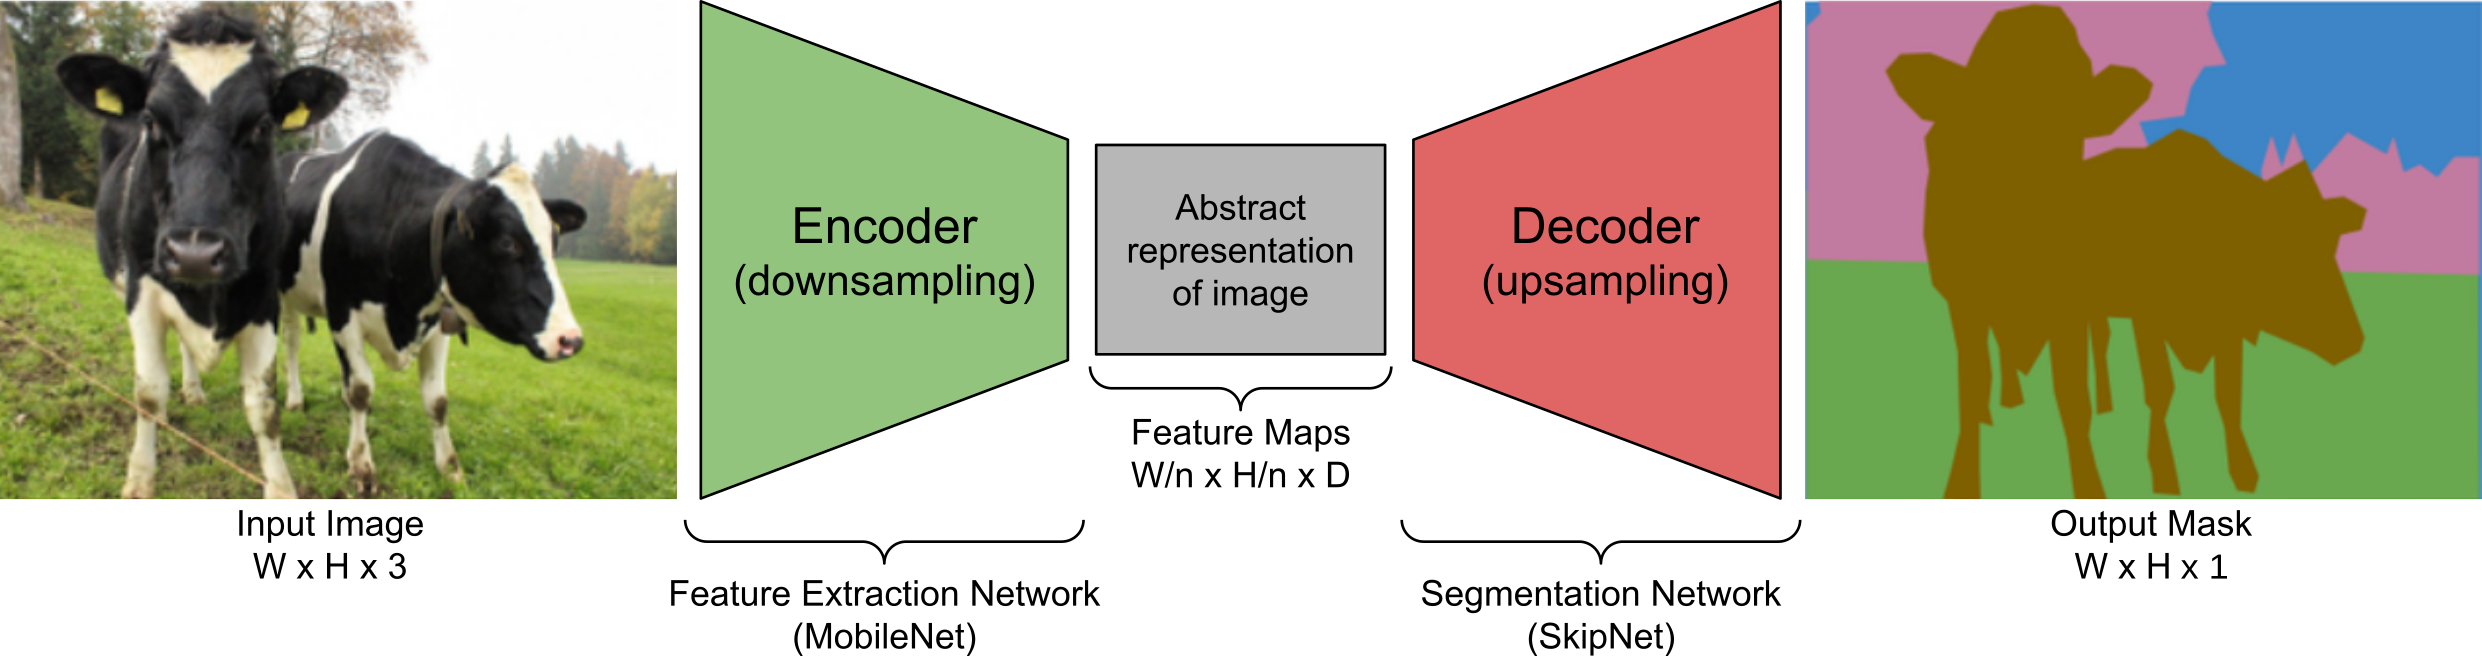
\includegraphics[width=12cm]{figures/Figure1.png}
	\caption{Esquema de la arquitectura de red FCN-MN utilizada en este trabajo, basada en la FCN propuesta por \citet{shelhamer2017fully}, reemplazando su encoder de extracción de features por las redes MobileNet \cite{howard2017mobilenets}, lo que produce features maps con un factor de downsampling n. Como decoder para la producción  del mapa de segmentación se utiliza la red SkipNet \cite{siam2018rtseg}, implementando las variantes 32s, 16s y 8s.}
	\label{fig:FCN-MN}
\end{figure}


Por otra parte, para recuperar la información espacial de grano fino perdida al avanzar a través de las capas del encoder, se suelen utilizar conexiones que sobrepasan al menos una capa de la red, llamadas \emph{skip connections}. Éstas se utilizan para transferir información espacial local desde las capas internas del encoder directamente a la entrada del decoder. En general, estas conexiones mejoran los resultados de segmentación, ya que mitigan la pérdida de información espacial permitiendo al decoder incorporar información de feature maps internos, aunque su impacto puede variar según la skip architecture que se proponga. En \citet{long2015fully} se proponen tres skip architectures: la 32s que no toma información de capas internas del encoder; la 16s que toma información espacial de grano-medio de capas profundas del encoder; y la 8s, que toma información espacial de grano-fino de capas menos profundas del encoder. Los detalles de estas arquitecturas quedan fuera del alcance de este trabajo, pero pueden consultarse en \citet{long2015fully} y \cite{shelhamer2017fully}. Dado que los resultados reportados en la literatura no son concluyentes respecto a que arquitectura es mejor \cite{long2015fully, shelhamer2017fully}, en este trabajo se consideran las tres alternativas.

A pesar de haber alcanzado excelentes resultados en la práctica,  estas arquitecturas conllevan una importante carga de recursos computacionales. Con esto en mente, en este trabajo se reemplazó el encoder VGG \cite{Simonyan2015VeryDC} propuesto originalmente por Long para las FCN, por la red MobileNet \cite{howard2017mobilenets}, una red que se destaca por tener tan solo 4.2 millones de parámetros frente a los 138 millones de parámetros de VGG, permitiendo que el proceso de entrenamiento y testeo sea considerablemente más rápido,  con requerimientos de memoria muy inferiores, pero manteniendo la performance. El uso de MobileNet como encoder en las FCN de \citet{long2015fully} no es novedoso, sino que ha sido ya propuesto para la arquitectura 8s por \citet{siam2018rtseg} en su arquitectura SkipNet. Técnicamente, la propuesta de \citet{siam2018rtseg} es sumamente sencilla, por lo que nos atrevemos aquí a extenderla a las arquitecturas 16s y 32s propuestas originalmente por \citep{long2015fully}. Debido a estos cambios es que nos referimos a estas redes como FCN-MN de aquí a lo que resta del paper.


%------------------


\subsubsection{Sliding Windows y Clasificador de patches (SW-C)}
\label{sec:sw}


En está seccion se describe el enfoque propuesto por \citet{perez2017image} para clasificación de imágenes de yema y una implementación del mismo para detección basada en sliding windows descrita en el trabajo original.

Este enfoque opera en tres pasos: (i) aplica el algoritmo de sliding windows sobre una imagen para extraer patches (sub-imágenes o regiones rectangulares); (ii) clasifica (todos los píxeles de) cada patch en yema o no-yema mediante el algoritmo presentado en \citet{perez2017image}; y (iii) produce la máscara de segmentación final mediante un esquema de votación. A continuación se dan los detalles de cada paso.
%
Las técnicas sliding windows comprenden una familia de algoritmos ampliamente utilizados en el pasado como parte de diversos enfoques para localización de objetos con bounding boxes \citep{divvala2009empirical, wang2009hog, chum2007exemplar, ferrari2007groups, dalal2005histograms, rowley1996human}. En estos algoritmos, cada imagen es escaneada densamente desde un extremo de la imagen (e.g. esquina superior izquierda) hasta el otro extremo (e.g. esquina inferior derecha) mediante una ventana deslizante rectangular en diferentes escalas y diferentes desplazamientos, extrayendo sub-imágenes o patches de la imagen original. En este trabajo, se definen 10 tamaños de ventana de igual alto y ancho, a saber 100, 200, 300, 400, 500, 600, 700, 800, 900 y 1000 píxeles, con un desplazamiento horizontal del $50\%$ el ancho de la ventana y un desplazamiento vertical del $50\%$ el alto de la ventana, lo que produce una superposición del $50\%$ entre parches contiguos. Estos valores se eligen sobre la base del análisis de robustez del clasificador que presenta \citet{perez2017image} para la geometría de la ventana. Este análisis muestra que el clasificador (explicado en la sección \ref{sec:swtrain}) es robusto para los patches que contienen al menos $60\%$ de los píxeles de una yema, y estos deben cubrir al menos el $20\%$ del patch. Los autores argumentan que un algoritmo de detección por sliding-windows podría proponer fácilmente un esquema para elegir el tamaño y el desplazamiento de la ventana que garantice que en algún punto del escaneo la ventana satisface los requerimientos de robustez. Sin embargo no se dan detalles de cómo implementarlo, por lo que en este trabajo solo nos limitamos a reportar resultados para tamaños fijos de ventana y desplazamiento explicados. Dado que las yemas del corpus tienen un diámetro en píxeles variable (correspondientes a parches que varían de 100×100 a 1600×1600 píxeles aproximadamente) no todos los tamaños de ventana podrán satisfacer los requerimientos de robustez para todos los patches, pero los resultados todavía pueden ser útiles a los efectos de realizar la comparación con el enfoque FCN-MN.
%
El segundo paso de este enfoque consiste en determinar si un patch es de clase yema o no-yema. El clasificador de \citet{perez2017image} toma los patches producidos por el sliding windows y para cada uno realiza las siguiente operaciones: (i) computa features visuales de bajo nivel mediante el algoritmo \emph{Scale Invariant Feature Transform} (SIFT) \cite{lowe2004distinctive}; (ii) construye un descriptor de alto nivel para cada patch empleando el algoritmo \emph{Bag of Features} (BoF) \cite{csurka2004visual} sobre los features SIFT del paso anterior; y (iii) determina la clase de cada patch usando el descriptor BoF sobre un clasificador construido mediante el algoritmo \emph{Support Vectors Machine} \cite{vapnik2013nature}. Los detalles del entrenamiento de este clasificador se posponen hasta la sección \ref{sec:swtrain} (Entrenamiento SW-C).

Finalmente, el tercer paso del enfoque consiste en construir la máscara binaria donde se encuentran etiquetados los píxeles que pertenecen a la clase yema y no-yema. Esta máscara es construida a través de un esquema de votación donde cada píxel suma un voto por cada patch que lo contiene clasificado como yema, el cual podría ser de un máximo de 4 para algunos píxeles debido a que el deslizamiento propuesto entre patches presenta solapamiento tanto horizontal como vertical. Luego, se establece un umbral de votos mínimos $\nu$ que puede tomar los valores del 1 al 4, de tal manera que los píxeles con una cantidad de votos igual o mayor a $\nu$ son clasificados como yema, caso contrario se clasifican como no-yema.

%------------------------
\subsection{Colección de imágenes}
\label{sec:corpus}

La colección de imágenes utilizada en este estudio consiste en la misma colección de imágenes utilizadas originalmente en \citet{perez2017image}, el cual se ha descargado de la URL indicada por los autores http://dharma.frm.utn.edu.ar/vise/bc. 
De las 760 imágenes de esta colección, se seleccionaron las 698 imágenes aquellas que contenían sólo una yema. Cada imagen está acompañada de una máscara con el ground truth, es decir la segmentación manual de la yema que contiene . Estas 698 imágenes y sus máscaras fueron empleadas durante el entrenamiento y evaluación de los dos enfoques propuestos. Para esto, el corpus de imágenes se separó en dos subconjuntos disjuntos: el \emph{trainset} con el $80\%$ de las imágenes y el \emph{testset} con el restante $20\%$. Esto resultó en un trainset de 558 imágenes y un testset de 140 imágenes, ambos con sus respectivas máscaras ground truth. De esta manera, los dos enfoques propuestos utilizan exactamente las mismas 558 imágenes durante el entrenamiento, y las mismas 140 imágenes durante la evaluación.

%---------------------------
\subsection{Entrenamiento de los modelos} 
\label{sec:train}

En esta sección se dan los detalles del proceso de entrenamiento para cada enfoque empleando las 558 imágenes del trainset.



\subsubsection{Entrenamiento enfoque FCN-MN.} 
\label{sec:fcntrain}

Para el entrenamiento de este enfoque se utilizaron las 558 imágenes reservadas para este propósito, las mismas que se usaron para el entrenamiento del enfoque anterior. Estas imágenes presentan diferentes resoluciones, sin embargo las FCN-MN requieren una entrada de tamaño fijo. Por esto, todas las imágenes (incluida sus máscaras) fueron escaladas a una resolución de $1024 \times 1024$ píxeles usando un método de interpolación bilinear \citep{han2013comparison}. Además, para las imágenes del trainset se realizó un scaling en los valores de intensidad RGB de los píxeles de [0,255] a [-1, 1].

Dado que la cantidad de imágenes en el trainset se considera escasa, para lograr un entrenamiento robusto se emplearon dos técnicas ampliamente utilizadas en la práctica: \emph{transfer learning} \cite{pan2009survey} y \emph{data augmentation} \cite{shorten2019survey}. El proceso de transfer learning se realizó de la siguiente manera: (i) se implementa la red MobileNet original propuesta en \citet{howard2017mobilenets}; (ii) se inicializa la red con los parámetros pre-entrenados sobre el dataset de benchmark ImageNet \cite{kornblith2019better}; (iii) se reemplaza la capa de clasificación multiclase de MobileNet por una capa de clasificación binaria; (iv) se entrena la red como un clasificador de patches yema y no-yema de forma análoga al entrenamiento de SVM, empleando el trainset de patches balanceado luego de escalar todas sus imágenes a $224 \times 224$ píxeles; y (v) se toman los parámetros obtenidos en este pipeline para inicializar el encoder de nuestra FCN-MN, introducido en la sección \ref{sec:fcn}. El proceso de data augmentation se aplicó on the fly durante el entrenamiento, i.e. en la medida que el proceso requería nuevas imágenes. Por cada imagen del traiset se generaron cientos de nuevas imágenes aplicando simultáneamente las siguientes siete operaciones, donde sus valores se tomaron de forma aleatoria con probabilidad uniforme: \emph{rotación} de hasta $45\degree$; \emph{traslación horizontal} de hasta $40\%$; \emph{traslación vertical} de hasta $40\%$; \emph{shear} de hasta $10\%$; \emph{Zoom} de hasta $30\%$; \emph{flip horizontal}; y \emph{flip vertical}. 
En general, para el entrenamiento de una FCN-MN se requiere especificar el \emph{método de optimización} y el valor de \emph{dropout}, dos parámetros típicamente definidos por el usuario. En este trabajo, los  métodos de optimización que se tuvieron en cuenta fueron Adam (con parámetros $Learning Rate = 0.001$, $beta1= 0.9$ y $beta2 = 0.999$), RMSProp (con parámetros $Learning Rate = 0.001$ y $rho = 0.9$) y Stochastic Gradient Descent (con parámetros $Learning Rate = 0.0001$ y $Momentum = 0.9$). Los valores de parámetros para RMSProp y Adam corresponden a los sugeridos en \cite{ruder2018gradientdescent}, mientras que para Stochastic Gradient Descent se establecieron valores de parámetros de manera que no dieran problemas durante el entrenamiento. Para el caso de dropout se definieron los valores $0.5$ y $0.001$, donde el primero es el estándar de facto y el segundo es tomado de forma arbitraria. La mejor combinación entre método de optimización y valor de dropout se estableció en tiempo de entrenamiento sobre un conjunto de validación, utilizando el enfoque \emph{4-fold cross validation} por 60 epochs, variando sobre los tres métodos de optimización y los dos valores de dropout. Los valores seleccionados fueron aquellos que maximizan el promedio de la Jaccard’s \emph{Intersection-over-Union} (IoU) \citep{jaccard1912distribution},  en los 4-folds sobre las 3 variantes, siendo IoU una medida de evaluación típica de problemas de segmentación (ver sección \ref{subsec:segmetrics}). Observamos en la Tabla \ref{tab:TablaX} que la combinación de parámetros con la que se alcanza mayor IoU promedio es RMSProp con dropout de $0.001$. 

\begin{table}[]
	 \resizebox{\textwidth}{!}{%
	\begin{tabular}{lll}
		\hline
		\multicolumn{1}{|l|}{} & \multicolumn{2}{c|}{\textbf{Mean IoU}} \\ \hline
		\multicolumn{1}{|c|}{\textbf{Optimizer}} & \multicolumn{1}{c|}{\textbf{Dropout = 0.001}} & \multicolumn{1}{c|}{\textbf{Dropout = 0.5}} \\ \hline
		RMSprop & {\ul 0.44253} & 0.3117 \\
		Adam & 0.240277 & 0.315714 \\
		SGD & 0.000886 & 0.00151 \\ \hline
	\end{tabular}}
	\caption{Promedio de IoU sobre las 3 variantes para cada combinación de parámetros.}
	\label{tab:TablaX}
\end{table}


Finalmente se procedió a entrenar las 3 variantes con RMSProp como método de optimización y un valor de dropout de $0.001$ sobre el conjunto de entrenamiento completo por 200 epochs.

\subsubsection{Entrenamiento enfoque SW-C} 
\label{sec:swtrain}


La etapa de entrenamiento para este enfoque se realiza de la misma manera que para el workflow original propuesto en \citet{perez2017image}. Esto implica entrenar un clasificador binario para que aprenda el concepto de yema versus no-yema a partir de un corpus de patches rectangulares que contienen o no una yema. Durante el entrenamiento, los patches yema deben ser regiones que circunscriben perfectamente la yema (ver FIGURA). Los patches no-yema deben ser regiones que no contienen ni un solo píxel de yema (ver FIGURA). Por lo tanto, para construir el corpus de patches, se procesaron las 558 imágenes y sus máscaras siguiendo el mismo protocolo que en \citet{perez2017image}, obteniendo un total de 558 patches que circunscriben a cada yema (existe una por imagen) y más de 25000 patches no-yema (el área no-yema es mucho mayor al área que ocupa una yema en la imagen). El tamaño de estos patches es variable, con resoluciones entre $0.1$ y $2.6$ megapíxeles aproximadamente (patches de $100 \times 100$ a $1600 \times 1600$ píxeles).

A partir de este corpus de patches, se creó un trainset de patches balanceado, i.e. con 558 patches de cada clase, donde los patches no-yema fueron tomados al azar entre miles de patches. El entrenamiento se realizó tal como se detalla en el pipeline propuesto en \citet{perez2017image}: (i) se extrajeron descriptores SIFT todos los patches del trainset; (ii) se aplicó BoF con tamaño de vocabulario igual a 25, dado que fue el modelo con mejores resultados según los autores; y (iii) se entrenó el clasificador SVM sobre los descriptores BoF de cada patch, empleando un kernel \emph{Radial Basis Function}, donde el valor de los parámetros $\gamma$ y $C$ se estableció mediante un 5-fold cross-validation sobre los mismos rangos de valores, i.e. $\gamma = \{2^{-14}, 2^{-13},\ldots, 2^{-7}\}$ y $C = \{2^{5}, 2^{6},\ldots, 2^{14}\}$.

%#######################################################################
%#######################################################################
\section{Experimental results} \label{sec:results}

In this section we present a systematic evaluation of the quality our proposed procedure FCN-MN for bud detections quality, which, 
%
according to the discussion in the introduction, can be decomposed on the three aspects that impact on the relevant bud related variables listed in Table 1: \emph{segmentation}, \emph{individualization}, and \emph{localization}. 

%
For that, we start in the following subsection by presenting metrics that quantify the quality for these aspects, followed by the results   subsection~\ref{sec:results} that presents details on the metric values obtained for different experiments over the test set of images. 


\subsection{Performance metrics}

% The main challenge for quantifying the errors for the three aspects of detection requires the understanding that the detection produced by both FCN-MN and SW algorithms consists of associating each \emph{connected component} of the output binary masks with one detected bud.


% Then, we refine the evaluation by reporting  the quality of the segmentation for those connected components that correctly detected a bud. We start in the following section by defining the metrics used to validate both detection and segmentation, and then proceed to compare the results of applying those metrics to the masks produced by our FCN-MN approach against those of the scanning windows approach of cite{perez2017image} (c.f. Section~\ref{sec:sw}), over all 140 images of the test corpus.


\subsubsection{Individualization metrics } \label{subsec:detectmetrics}

Individualization of buds, in both FCN-MN and SW, is the result of two steps: (i)  the thresholding of the algorithm’s output mask into a \emph{binary mask}, keeping all pixels of $\nu$ the probabilistic mask output by FCN-MN with values higher than $\tau$ and keeping all pixels belong to at least $\nu$ patches rendered positive by SW, and (ii) the association of each \emph{connected component} of the binary mask to exactly one (detected) bud. 

%
An incorrect individualization is thus the result of incorrect matching of detected components with actual buds in the image. This matching can get very complicated when there is an unknown number of true buds in the scene as can be seen by the large amount of possible detection metrics defined in \cite{oguz2017dice}. To simplify the analysis our image corpus contains a single bud per image, avoiding the need of all metrics that report the confusing situation of a component overlapping more than one true bud. This results in the following simplified list of possible metrics:

\begin{itemize}
	\item \textbf{Correct Detection} ($CD$) is the best case, and counts all images in the test corpus for which the detected binary mask presents a single connected component, and this connected component overlaps with the true bud of the image. This would correspond with a \emph{true positive} situation.
	\item \textbf{Split} ($S$) occurs when there is more than one detection per bud, which happens  when the mask contains multiple connected components, all of which overlaps the true bud. This metric counts the total number of such components over all images in the test corpus.
	\item \textbf{False Alarm} ($S$), is equivalent to a \emph{false positive} situation, and corresponds to connected components not overlapping with the true bud. As for splits, it counts, for each image, the number of such components.
	\item \textbf{Detection Failure} ($DF$), is equivalent to a \emph{false negative} situation,when the detection mask presents no connected components. It counts one each image satisfying this condition.
\end{itemize}

All four of these cases are mutually exclusive, that is, no image can satisfy any two (or more) of these definitions simultaneously. To quantify the individualization quality one could simply report these quantities counted over the test set, with the best case consisting in a $CD$ value equal to the cardinality of this set. However, determining the overall individualization quality from the analysis of $4$ quantities can get rather complicated. 
%
One alternative is reporting the well-known \emph{precision} and \emph{recall} together with the \emph{F1-measure} computed as their harmonic average \( 2 \times \frac{precision \times recall}{precision + recall}\). For that, we have to address first the fact that  we have two differing true positive counts: $CD$ and $S$. We solve this by first counting as true positives not only the $CD$ type of images, but the $S$ ones, i.e., we count as one true positive any image with either a correct detection or a split case, resulting in:

\begin{equation}
detection \mbox{-} precision = \frac{true\ positives}{true\ positives+false\ positives} \\
= \frac{CD+S}{CD+S+FA}
\label{eq:detection-precision}
\end{equation}

\begin{equation}
detection \mbox{-} recall = \frac{true\ positives}{true\ positives+false\ negatives} \\
= \frac{CD+S}{CD+S+DF},
\label{eq:detection-recall}
\end{equation}

and then account for the split type of errors by reporting  the percentage of all true positives that resulted in splits, which requires no specific metric. 

\subsubsection{Segmentation metrics} \label{subsec:segmetrics}

Individualization metrics, although informative, relies on  the overlap between the detected and true buds, regardless of how minimal the overlap. This could miss several possible pixelwise detection errors, resulting in rather coarse comparisons between competing detection algorithms. For instance, a correct detection could present a very small overlap with the true bud, with many or even a majority of the true bud’s pixels missing (i.e., several \emph{false negatives} pixels), or could be erroneously reporting several pixels as bud pixels (i.e., several \emph{false positives} pixels). Clearly, the best case scenario would be a case of correct detection with no false negative or positive pixels, that visually would correspond to a perfect overlap of the detected connected component and the true bud.  Similarly, a pixel wise comparison of the masks could help assess the quality of the splits. The best split, for instance, would be one completely enclosed within the true mask, i.e., with none of its connected components presenting false positive pixels; while covering as much of the true bud mask as possible, i.e., presenting just enough false negatives to disconnect its components. 
%
Finally, a false alarm case, clearly presenting only false positive pixels, could be further assessed by the number of (false positive) pixels in its components. 

The community has proposed several metrics to quantify segmentation errors. The most obvious ones are those that 
report the \emph{fraction} of the whole image corresponding to \emph{true positive} pixels, denoted $TPF$; \emph{false positive} pixels,  denoted $FPF$;  and \emph{false negative} pixels, denoted $FNF$. 
%
As for the individualization metrics, one can simplify the analysis by considering the  pixelwise \emph{precision}  and \emph{recall}: 

\begin{eqnarray} 
segmentation\-precision &=& TPF / (TPF + FPF) \\
segmentation\-recall &=& TPF / (TPF + FNF)
\end{eqnarray}
% Another combination of these quantities, useful to assess the relative size of the false positives, is the \emph{false-positive-rate}, computed as $FPF/(FPF + TNF)$, or simply $FPF / NF$, where the latter is the fraction of negatives, that is, all except the true bud pixels. 
% But even these two quantities can be simplified into a single quantity in two different ways. accompanied by their weighted harmonic mean, the well-known \emph{F-measure}, 

\begin{equation} 
2 \times precision \times recall / (precision + recall),
\end{equation}

proposed independently by \citet{dice1945measures}, thus usually referred to as the \emph{Dice measure}. A common alternative to the Dice measure is the  Jaccard’s \emph{intersection-over-union} \citep{jaccard1912distribution}, 
equivalent to $TPF / (TPF+FPF+FNF)$. 

With these metrics, one could quantify the refinements discussed in the first paragraph above, by simply applying them, no to the whole mask, but to the individual individualization cases. For instance, reporting the mean Dice measured over all correctly detected components; or, to refine the assessment of how bad is a split, one could report the mean Dice measure to all components of some split, or the mean Dice measure over all split components of all split images. 

The case of false alarms is rather monotonous and not very informative, with zero precision and recall for all such components. Indeed, a pixelwise assessment of the gravity of a false alarm requires a quantification of the number of false positive pixels. One could simply consider the $FPF$, the fraction of all the image pixels that are false positives. Instead, we considered a normalization against the size of the bud to be more informative, resulting in the \emph{normalized área}(\textbf{NA}):

\begin{description}
	\item[Normalized Area ($NA$)]: the total área (i.e., number of pixels) of the component, normalized by the area of the true bud. 
\end{description}

%One could report the mean \emph{false-positive-rate} , computed as $FPF/(FPF + TNF)$, or simply $FPF / NF$, over all images, to assess the gravity of the false alarm components produced by some algorithm.  This qua

% Segmentation results for correct detection and splits allowed us to further assess the quality of the detections. However, as shown by the detection precision and recall results above, there is no lack of false detections, the false positive components we called false alarms. For instance, in their best versions, $2.3\%$ of all components produced by the FCN with threshold $0.8$ and architecture 16s are false alarms, increasing to $33\%$ for the case of SW with voting threshold 1 and windows size 1000px.  These percentages, however, do not tell us how bad these false alarms are. Whether they are large or small, or whether they are located nearby the true bud (appearing more as splits than false alarms) or they are further away. 

\subsubsection{Localization metrics} \label{subsec:locmetrics}

As a localization metric we propose the \emph{normalized distance} (\textbf{ND}), defined formally as:

\begin{description}
	\item[Normalized Distance ($ND$)]:  the distance between the center of mass of the component to the center of mass of the true bud, divided by the diameter of the true bud (defined as the maximum distance between any two border points of the true bud).
\end{description}


%%%%%%%%%%%%%%%%%%%%%%%%%%%%%%%%%%%%%%%%%%%%%%%%%%
%%%%%%%%%%%%%%%%%%%%%%%%%%%%%%%%%%%%%%%%%%%%%%%%%%

\subsection{Resultados Sistemáticos}   \label{sec:resultados}

We proceed now to assess the validity of our main hypothesis, namely, that FCN-MN is a better detector than its SW counterpart over each of the metrics defined in the previous section. 

For a thorough comparison we considered several cases for each algorithm, training $27$ FCN-MN detectors and $40$ SW detectors over the training set of $558$ images, one for each combination of their respective hyper-parameters. For FCN-MN these hyper-parameters are the three architectures 8s, 16s, and 32s, and the $9$ values $\{0.1, 0.2, \ldots, 0.9\}$ for the binarization threshold $\tau$; whereas for SW these hyper-parameters are the $10$ patch sizes $\{100, 200, \ldots, 1000\}$  and the $4$ values $\{1, 2, 3, 4\}$  of the voting threshold $\nu$.


Table \ref{tab:TablaXX} shows the results for the best detectors of each algorithm, reporting all performance metrics of the three aspects of detection: individualization, segmentation and localization. The first column shows the label of the selected detectors, with the subscript indicating the architecture and patch size for the case of FCN-MN and SW, respectively, while the superscript indicating the thresholds $\tau$ and $\nu$, respectively.

A detector was considered for inclusion in the table if, when compared to its counterparts of the same algorithm, it resulted in the higher value for at least one of the metrics, marked in bold in the table. For instance, the detectors FCN-MN$_{16s}^{0.8}$ SW$_{1000}^1$ are included because their precision is $97.7$ and $67.0$, respectively; the former being the largest among all $27$ FCN-MN detectors, and the latter being the largest  among the $40$ SW detectors. 

The individualization metrics reported are the \emph{detection-precision} labeled Prec, \emph{detection-recall} labeled Rec, \emph{F1-measure} labeled F1, and the total count of split components. All of these are computed from the quantities $CD$, $S$, $FA$ and $DF$, which are counted over all images in the test set; thus producing a single metric per detector.

For segmentation, the reported metrics are the \emph{segmentation-precision} labeled Prec, \emph{segmentation-recall} labeled Rec, and the \emph{Dice measure} labeled Dice. For the correctly detected group, the corresponding cell reports the mean value of the measures computed for each correctly detected test image, i.e., each image with only one component overlapping the true bud, with the corresponding standard deviation  in parenthesis. The same metrics are reported for the split group, where the mean and standard deviation are computed over the measures computed only for the split images, i.e., over the images containing at least two components overlapping the true bud. Here, the segmentation metrics are computed over the union of all split components (with the other, discarded alternative, being the mean metric over each split component) . 

For the false alarms we also reported a segmentation metric, the mean \emph{normalized area}($NA$), in this case computed individually for each false alarm component, reporting at each cell its mean over all false alarm component of all test images. 

Finally, for localization we report the \emph{normalized distance}($ND$) only for false alarms, considering that correctly detected and splits, as they overlap the true bud, should be close enough to render it unnecessary further analysis. Instead, a false alarm can be arbitrarily far from the true bud.  We thus report the mean $ND$ of each false alarm connected component that appears in any test image.

The table shows a clear improvement of FCN-MN over SW. For all metrics it is the case that the best  FCN-MN detector (bolded) improves (or ties) over the best SW detector (bolded); represented in the table by underlying the one with better metric; with the exception of the two segmentation recalls (for correctly detected and splits) for which the SW case has a better (larger) mean, $98.8$ versus $99.9$ for correctly detected, and $74.7$ versus $78.6$ for the split case; and the total split count $S$, with the best case for FCN-MN being $1$ and $0$ for the best SW case. These improvements are not statistically significant, however, due to the large standard deviations of the FCN-MN cases, of $3.4$ and $8.1$, for the correctly detected and split cases, respectively,  resulting in (statistically) overlapping values. 
%
In some cases the improvements of FCN-MN over SW are overwhelming. For instance, for the detection-precision, the correctly detected segmentation-precision, and the split segmentation-precision, the FCN-MN over SW improvements are $97.7$ versus $67.0$, $98.1$ versus $46.5$ and $99.9$ versus $67.5$, respectively.  Also, for $NA$ and $ND$ the  FCN-MN versus SW improvements are $0.04$ versus $0.22$, and $1.1$ versus $6.0$, respectively.

When analyzing FCN-MN for its own merits, one can observe rather high values for all metrics, reaching detection-precision of $97.7$ and detection-recall of $100$; and segmentation-precision and segmentation-recall for correctly detected of $98.1(0.6)$ and $98.8(3.4)$, respectively; and for splits $99.9(0.1)$ and $74.7(28.1)$, respectively. Also, for $NA$ the best values being $0.04(0.09$ and for $ND$ values as small as $0.04 (0.22)$.  
%
However, these quantities are all for different FCN-MN detectors. A better assessment must 
be conducted for one single detector. For that, we picked FCN-MN$_{16s}^{0.6}$. This detector reaches detection precision and recall of $95.6$ and $93.6$ respectively, meaning than only $4.4\%$ of all the detected connected components over all test images are false alarms, and that only $6.4\%$ of all true buds could not be detected (i.e., resulted in detection failure).
%
Also, only $3$ of all detections were splitted, which on average has a segmentation precision of $99.4(0.6)$ and segmentation recall of $16.2(10.6)$. The recall is rather small, suggesting that the split is in fact the result of  pixel wise detection of the bud so sparse that it got disconnected. In contrast, all remaining detections were correct (i.e., not splitted), reaching segmentation precisions of $92.2(8.7)$, a rather similar value to that of splits, but a much larger mean segmentation recall of $88.2(13.3)$. Overall, this resulted in a mean Dice measure for the correctly detected of $89.1(10.7)$; demonstrating a considerable (mean) coverage of the true bud, with only $10.9 \%$ of the buds pixels missing (on average), and only $11.8\%$ of the detected pixels covering the background (on average). 
%
But more promising are the false alarm results, showing that these components are rather small, covering only an area that is $8\%$ in size of the total area of a bud (on average), and distant to the true bud by only $1.1 (0.65)$ diameters. These small numbers suggest two things. First, due to their closeness to the true bud, the obvious closeness of the correctly detected and split components, and the fact that buds in real plants are typically tens or even hundreds of bud diameters apart, a simple spatial clustering of the components (a natural post-processing of our approach) would connect all these components together as one single, and correct, bud detection. Second, due to their small area, if clustered together, the false alarm components would only slightly reduce the segmentation precision. 

\begin{table}[]
	\tiny
	\centering		
	\begin{adjustbox}{angle=90}
		\resizebox{.9\textheight}{!}{%	
		\begin{tabular}{lllllllllllll}
			\hline
			\multicolumn{1}{|c|}{\textbf{}} & \multicolumn{5}{c|}{\textbf{Individualization metrics}} & \multicolumn{7}{c|}{\textbf{Segmentation metrics}} \\ \hline
			\multicolumn{1}{|c|}{\textbf{Model}} & \multicolumn{1}{c|}{\textbf{Prec}} & \multicolumn{1}{c|}{\textbf{Rec}} & \multicolumn{1}{c|}{\textbf{F1}} & \multicolumn{1}{c|}{\textbf{S}} & \multicolumn{1}{c|}{\textbf{ND}} & \multicolumn{1}{c|}{\textbf{CD-Prec}} & \multicolumn{1}{c|}{\textbf{CD-Rec}} & \multicolumn{1}{c|}{\textbf{CD-Dice}} & \multicolumn{1}{c|}{\textbf{S-Prec}} & \multicolumn{1}{c|}{\textbf{S-Rec}} & \multicolumn{1}{c|}{\textbf{S-Dice}} & \multicolumn{1}{c|}{\textbf{RA}} \\ \hline
			$FCN-MN_{8s}^{0.5}$ & 75,4 & 98,6 & 85,4 & 2 & 3,72 (4,64) & 91,0 (11,3) & 90,2 (11,7) & \cellcolor[HTML]{81D41A}{\ul \textbf{89,6 (10,3)}} & 96,6 (2,2) & 73,1 (17,6) & \cellcolor[HTML]{81D41A}{\ul \textbf{82,1 (10,2)}} & 0,26 (0,69) \\
			$FCN-MN_{8s}^{0.9}$ & 90,1 & 97,1 & 93,5 & 8 & 3,8 (5,66) & \cellcolor[HTML]{81D41A}{\ul \textbf{98,1 (6,0)}} & 68,3 (21,1) & 77,9 (19,6) & 98,7 (3,0) & 57,4 (18,4) & 70,8 (13,6) & 0,24 (0,5) \\
			$FCN-MN_{16s}^{0.1}$ & 71,3 & \cellcolor[HTML]{81D41A}{\ul \textbf{100}} & 83,2 & 6 & 5,27 (6,53) & 75,7 (13,1) & 95,4 (14,7) & 83,1 (13,5) & 83,1 (8,9) & 54,1 (21,9) & 61,9 (17,5) & 0,12 (0,44) \\
			$FCN-MN_{16s}^{0.4}$ & 87,0 & 96,4 & 91,5 & \cellcolor[HTML]{81D41A}\textbf{1} & 3,8 (5,08) & 87,7 (12,1) & 89,8 (18,2) & 87,0 (15,6) & 96,7 (0,0) & 37,0 (0,0) & 53,5 (0,0) & \cellcolor[HTML]{81D41A}{\ul \textbf{0,04 (0,09)}} \\
			$FCN-MN_{16s}^{0.6}$ & 95,6 & 93,6 & 94,6 & 3 & \cellcolor[HTML]{81D41A}{\ul \textbf{1,1 (0,65)}} & 92,2 (8,7) & 88,2 (13,3) & 89,1 (10,7) & 99,4 (0,6) & 16,2 (10,6) & 26,6 (16,8) & 0,08 (0,11) \\
			$FCN-MN_{16s}^{0.8}$ & \cellcolor[HTML]{81D41A}{\ul \textbf{97,7}} & 92,1 & \cellcolor[HTML]{81D41A}{\ul \textbf{94,9}} & 4 & 1,28 (0,95) & 95,8 (7,0) & 81,6 (14,6) & 87,0 (10,7) & 99,7 (0,3) & 34,2 (32,6) & 43,9 (33,1) & 0,1 (0,12) \\
			$FCN-MN_{16s}^{0.9}$ & \cellcolor[HTML]{81D41A}{\ul \textbf{97,7}} & 91,4 & 94,5 & 4 & 1,33 (0,9) & 97,6 (5,6) & 74,5 (16,5) & 83,1 (12,8) & \cellcolor[HTML]{81D41A}{\ul \textbf{99,9 (0,1)}} & 31,8 (27,9) & 41,6 (34,0) & 0,07 (0,11) \\
			$FCN-MN_{32s}^{0.1}$ & 35,4 & \cellcolor[HTML]{81D41A}{\ul \textbf{100}} & 52,2 & 8 & 4,62 (5,59) & 67,4 (14,0) & \cellcolor[HTML]{81D41A}\textbf{98,8 (3,4)} & 79,1 (11,0) & 86,0 (9,4) & 73,4 (19,6) & 77,1 (10,4) & 0,14 (0,66) \\
			$FCN-MN_{32s}^{0.2}$ & 50,9 & \cellcolor[HTML]{81D41A}{\ul \textbf{100}} & 67,5 & 10 & 4,33 (6,17) & 73,9 (13,6) & 98,1 (3,8) & 83,5 (10,1) & 92,2 (5,4) & 53,4 (25,8) & 63,6 (19,3) & 0,17 (0,55) \\
			$FCN-MN_{32s}^{0.3}$ & 49,8 & \cellcolor[HTML]{81D41A}{\ul \textbf{100}} & 66,5 & 10 & 3,68 (5,62) & 79,1 (13,2) & 95,5 (10,5) & 85,2 (11,8) & 88,5 (9,7) & 61,0 (35,1) & 65,8 (28,2) & 0,1 (0,39) \\
			$FCN-MN_{32s}^{0.6}$ & 68,5 & 99,3 & 81,1 & 16 & 2,95 (4,36) & 89,0 (11,5) & 89,1 (11,3) & 88,1 (9,6) & 92,4 (7,7) & \cellcolor[HTML]{81D41A}\textbf{74,7 (28,1)} & 78,1 (24,0) & 0,11 (0,3) \\
			$SW_{100}^{1}$ & \textbf{9,4} & \cellcolor[HTML]{E0C2CD}{\ul \textbf{100}} & \textbf{17,2} & 28 & 7,68 (6,02) & 24,6 (17,7) & 86,7 (19,5) & 33,6 (15,1) & 57,9 (28,2) & 24,8 (16,8) & 27,9 (13,8) & 1,08 (3,2) \\
			$SW_{100}^{3}$ & 14,6 & 93,1 & 25,3 & 40 & 6,45 (6,19) & 42,4 (26,4) & 56,8 (29,9) & \cellcolor[HTML]{E0C2CD}\textbf{39,9 (19,7)} & 55,5 (32,2) & 24,8 (18,1) & 26,0 (15,6) & 0,31 (0,96) \\
			$SW_{100}^{4}$ & 19,5 & 87,4 & 31,9 & 49 & \cellcolor[HTML]{E0C2CD}\textbf{6,0 (6,56)} & \cellcolor[HTML]{E0C2CD}\textbf{46,5 (29,3)} & 39,2 (28,9) & 33,9 (21,1) & 49,0 (29,0) & 20,1 (13,7) & 24,1 (14,0) & \cellcolor[HTML]{E0C2CD}\textbf{0,22 (0,57)} \\
			$SW_{200}^{1}$ & 20,0 & \cellcolor[HTML]{E0C2CD}{\ul \textbf{100}} & 33,3 & 12 & 7,56 (5,35) & 16,6 (12,5) & 94,9 (13,5) & 25,9 (14,2) & 49,3 (26,4) & 40,2 (17,4) & 36,8 (11,9) & 5,13 (19,3) \\
			$SW_{200}^{3}$ & 26,0 & 98,6 & 41,1 & 19 & 8,94 (6,22) & 29,9 (17,0) & 74,7 (27,3) & 38,5 (17,0) & \cellcolor[HTML]{E0C2CD}\textbf{67,5 (32,7)} & 16,5 (8,9) & 24,2 (11,9) & 1,69 (3,15) \\
			$SW_{300}^{1}$ & 26,9 & \cellcolor[HTML]{E0C2CD}{\ul \textbf{100}} & 42,4 & 2 & 6,83 (4,44) & 13,7 (13,6) & 97,0 (9,6) & 21,6 (15,5) & 55,0 (11,8) & 48,1 (1,1) & \cellcolor[HTML]{E0C2CD}\textbf{50,8 (4,5)} & 7,79 (20,5) \\
			$SW_{400}^{1}$ & 32,7 & \cellcolor[HTML]{E0C2CD}{\ul \textbf{100}} & 49,3 & 2 & 7,12 (4,15) & 10,5 (11,7) & 98,7 (9,3) & 17,2 (15,3) & 42,6 (10,1) & 61,9 (11,6) & 50,4 (10,9) & 11,59 (24,05) \\
			$SW_{400}^{2}$ & 34,6 & \cellcolor[HTML]{E0C2CD}{\ul \textbf{100}} & 51,4 & 4 & 7,88 (4,89) & 15,6 (15,1) & 94,5 (13,3) & 23,8 (15,6) & 48,7 (27,6) & 36,0 (4,6) & 38,6 (13,1) & 9,54 (26,13) \\
			$SW_{500}^{1}$ & 40,2 & \cellcolor[HTML]{E0C2CD}{\ul \textbf{100}} & 57,3 & 1 & 7,22 (4,04) & 8,40 (9,7) & \cellcolor[HTML]{E0C2CD}{\ul \textbf{99,9 (4,9)}} & 14,2 (13,8) & 17,9 (0,0) & \cellcolor[HTML]{E0C2CD}{\ul \textbf{78,6 (0,0)}} & 29,2 (0,0) & 17,39 (30,07) \\
			$SW_{500}^{2}$ & 38,6 & \cellcolor[HTML]{E0C2CD}{\ul \textbf{100}} & 55,7 & 1 & 7,56 (4,42) & 13,5 (14,0) & 95,2 (14,5) & 21,0 (16,0) & 35,2 (0,0) & 45,9 (0,0) & 39,8 (0,0) & 17,19 (39,07) \\
			$SW_{600}^{1}$ & 43,5 & \cellcolor[HTML]{E0C2CD}{\ul \textbf{100}} & 60,6 & \cellcolor[HTML]{E0C2CD}{\ul \textbf{0}} & 7,72 (4,3) & 6,9 (7,8) & 98,5 (10,7) & 12,0 (12,0) & nan (nan) & nan (nan) & nan (nan) & 25,48 (48,45) \\
			$SW_{600}^{2}$ & 41,7 & \cellcolor[HTML]{E0C2CD}{\ul \textbf{100}} & 58,8 & 1 & 7,92 (4,38) & 10,4 (10,6) & 93,7 (18,9) & 17,2 (14,4) & 19,7 (0,0) & 27,2 (0,0) & 22,9 (0,0) & 20,41 (38,32) \\
			$SW_{700}^{1}$ & 50,6 & \cellcolor[HTML]{E0C2CD}{\ul \textbf{100}} & 67,2 & \cellcolor[HTML]{E0C2CD}{\ul \textbf{0}} & 7,75 (4,45) & 5,6 (6,5) & 98,6 (12,0) & 9,9 (10,3) & nan (nan) & nan (nan) & nan (nan) & 31,95 (64,36) \\
			$SW_{800}^{1}$ & 56,7 & \cellcolor[HTML]{E0C2CD}{\ul \textbf{100}} & 72,4 & \cellcolor[HTML]{E0C2CD}{\ul \textbf{0}} & 7,7 (4,06) & 5,1 (6,6) & 97,7 (11,0) & 9,0 (10,4) & nan (nan) & nan (nan) & nan (nan) & 44,53 (71,52) \\
			$SW_{800}^{2}$ & 49,6 & 99,2 & 66,1 & \cellcolor[HTML]{E0C2CD}{\ul \textbf{0}} & 7,82 (4,1) & 8,3 (9,4) & 95,0 (15,9) & 13,9 (13,2) & nan (nan) & nan (nan) & nan (nan) & 30,52 (46,45) \\
			$SW_{900}^{1}$ & 64,3 & \cellcolor[HTML]{E0C2CD}{\ul \textbf{100}} & 78,3 & \cellcolor[HTML]{E0C2CD}{\ul \textbf{0}} & 7,9 (4,35) & 4,2 (5,7) & 94,7 (19,0) & 7,5 (9,2) & nan (nan) & nan (nan) & nan (nan) & 48,16 (80,31) \\
			$SW_{900}^{3}$ & 42,2 & 92,4 & 58,0 & \cellcolor[HTML]{E0C2CD}{\ul \textbf{0}} & 7,65 (4,67) & 15,0 (14,8) & 81,5 (28,9) & 22,7 (16,8) & nan (nan) & nan (nan) & nan (nan) & 17,97 (29,56) \\
			$SW_{1000}^{1}$ & \cellcolor[HTML]{E0C2CD}\textbf{67,0} & \cellcolor[HTML]{E0C2CD}{\ul \textbf{100}} & \cellcolor[HTML]{E0C2CD}\textbf{80,2} & \cellcolor[HTML]{E0C2CD}{\ul \textbf{0}} & 7,91 (4,3) & 3,7 (4,7) & 95,3 (18,3) & 6,8 (7,9) & nan (nan) & nan (nan) & nan (nan) & 57,83 (84,87) \\
			$SW_{1000}^{2}$ & 56,7 & 98,3 & 71,9 & \cellcolor[HTML]{E0C2CD}{\ul \textbf{0}} & 7,98 (4,44) & 6,3 (6,9) & 93,8 (19,1) & 11,1 (10,9) & nan (nan) & nan (nan) & nan (nan) & 47,26 (68,92) \\ \hline
		\end{tabular}}
	\end{adjustbox}
	\caption{Individualization, segmentation and localization metrics for the best FCN-MN and SW detection models. Bolded cells denote the best among all the cells in the column corresponding to the same algorithm (i.e., the best among FCN-MN, and the best among SW). Underlined (bolded) cells denote the best overall FCN-MN and SW detection models.}
		
		\label{tab:TablaXX}
	\end{table}


%#######################################################################
%#######################################################################
\subsubsection{Detailed analysis of individualization metrics} 
\label{sub:compFCNSW}

% We start by reporting the comparison of detection-precision and detection-recall, to then analyze how many of the true positives involved are indeed splits.  

Graphically one could expect a better combined analysis of the detection-precision and detection-recall than one could obtain by comparing the F1-measure. This is shown as a scatter plot in Figure~ref{fig:detection-scatter-plot}, a graphical representation of a non-summarized version of the second and third columns of Table~\ref{tab:TablaXX}. Each dot  in the plot is located according to the detection-precision and detection-recall, and the colored black or white whether it corresponds to an FCN-MN or an SW detection model.
%
The graph reinforces the clear and undisputed improvements of FCN-MN over SW already detected in the table, with similar detection-recalls but larger detection-precisions over the majority of scenarios, resulting in a larger area under the PR curve. 

 \begin{figure}
	\centering
	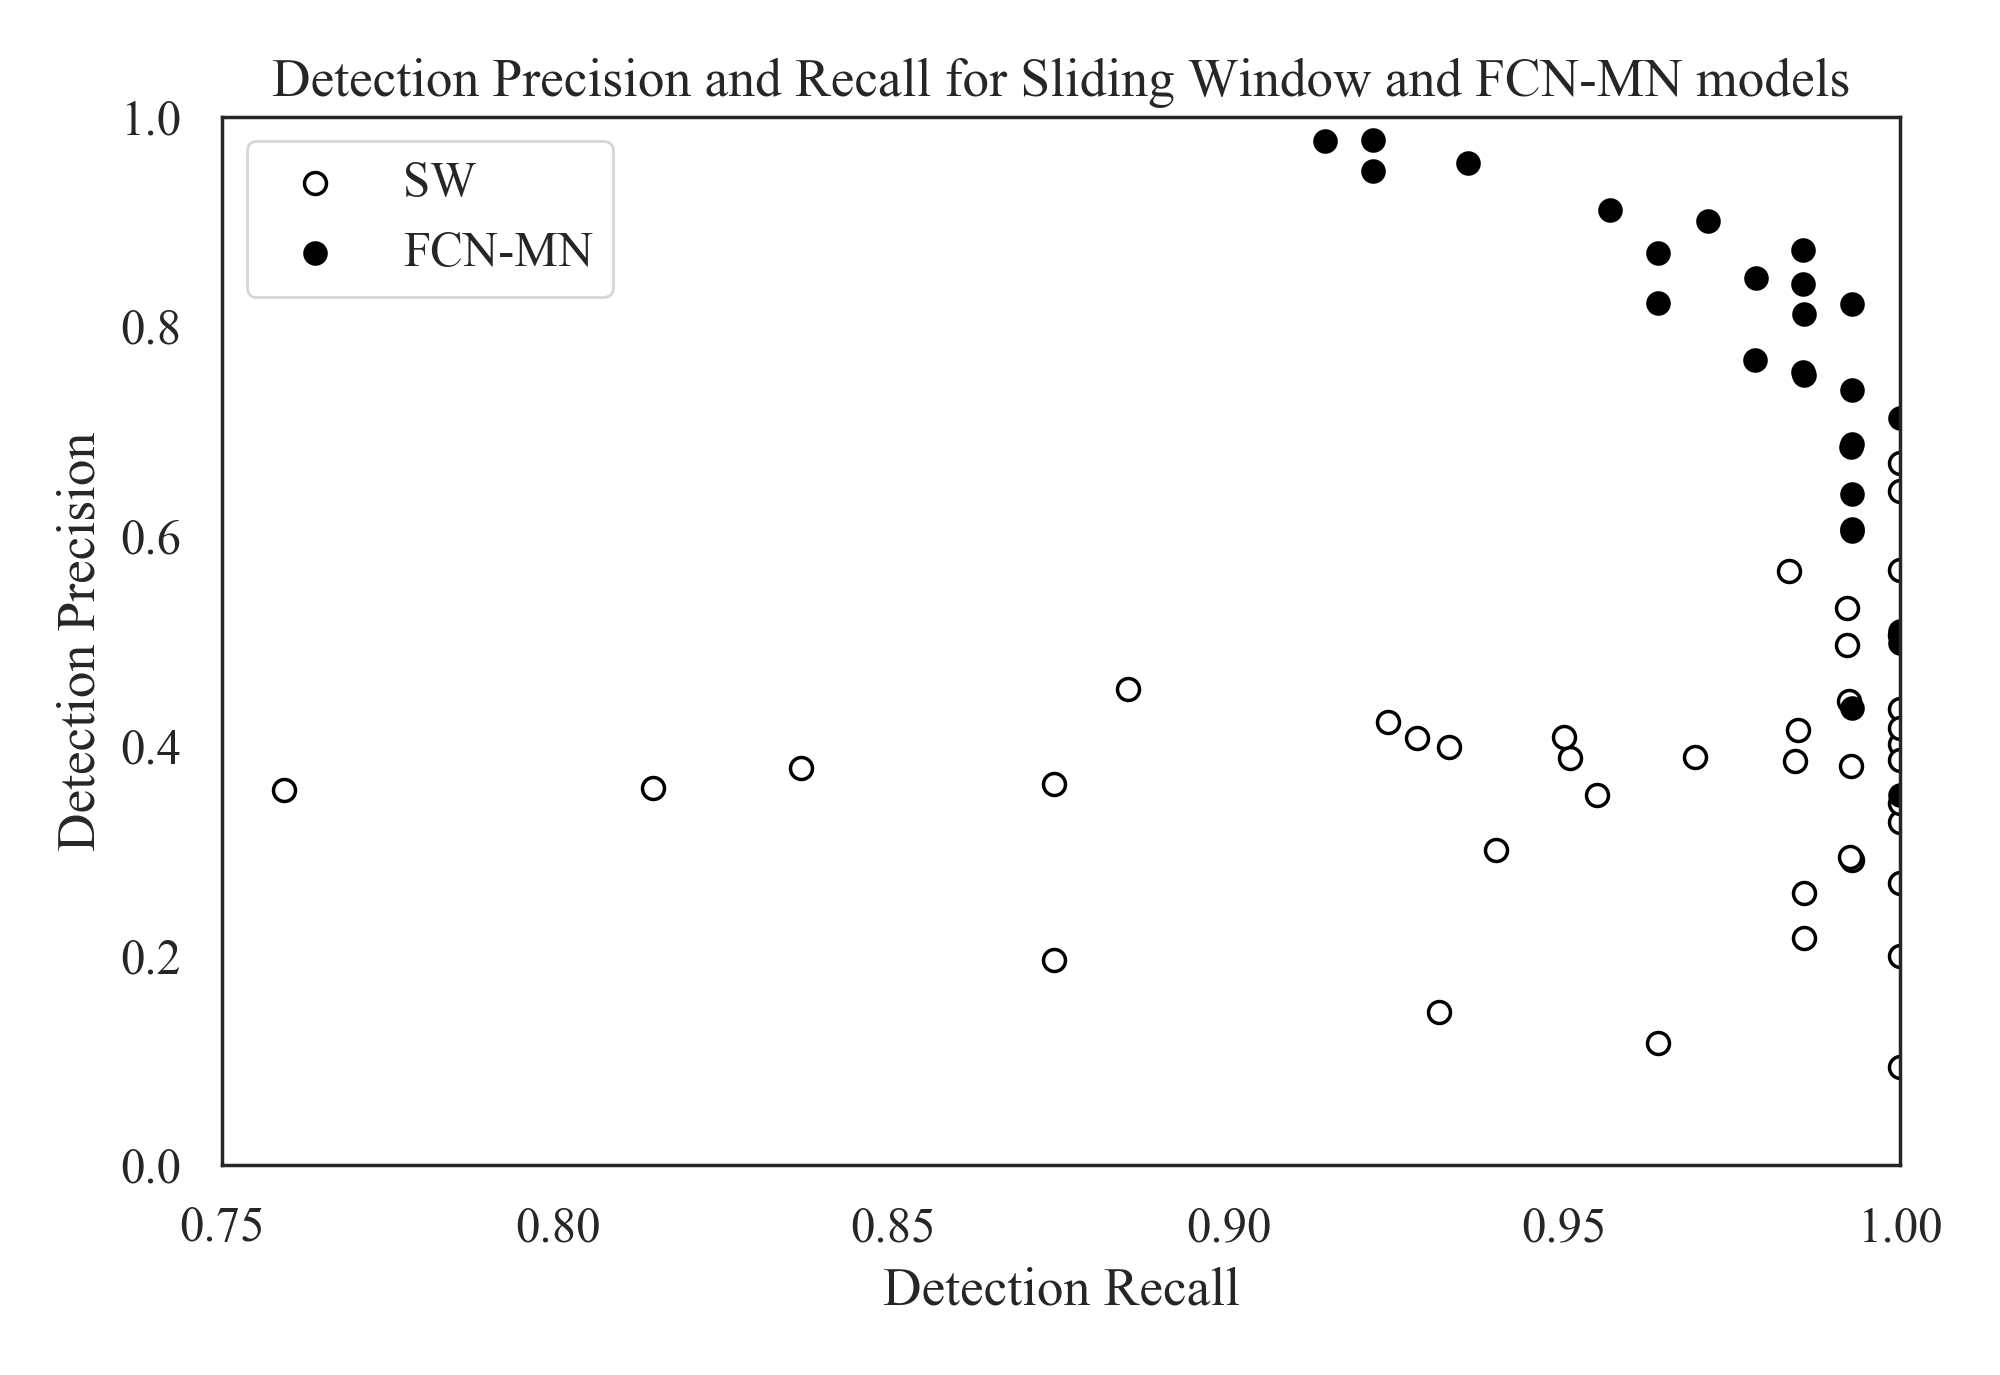
\includegraphics[width=\textwidth]{figures/111_precision_recall_detection.png}
	\caption{Precision-Recall scatterplots of the second and third columns of Table~\ref{tab:TablaXX} discriminating the results for FCN-MN and SW with black and white dots, respectively. Each dot then  represents the detection-precision and detection-recall computed over all images of the tests, for some particular  configurations of hyperparameters. For FCN-MN, these would be the architecture, with values 8s, 16s and 32s, and threshold $\tau = \{0.1, 0.2, \ldots, 0.9\}$,  for a total of $27$ black dots; while for SW these would be the patch sizes  $\{100, 200, \ldots, 1000\}$ and voting thresholds $\{1, 2, 3, 4\}$, for a total of a total of 40 white dots.}
	\label{fig:detection-scatter-plot}
\end{figure}

Detection-precision and detection-recall are computed over a combination of correctly detected and splitted components. To easily assess the impact of the split cases, we show in Figure \ref{fig:number-of-split} the $S$ values, corresponding to  the fifth column of a   (non-summarized version of) Table~\ref{tab:TablaXX} in the form of a histogram; with bins representing values of $S$,  and the bars for that bin representing the proportion of models that resulted in that value of $S$. Black and white bars discriminate the cases for FCN-MN and SW, respectively. For instance, the first bin indicates that approximately $54\%$ of the FCN-MN models and approximately $62\%$ of the SW models resulted in a total number splits of less than $5$. Overall, the FCN-MN distribution is slightly more concentrated in the lower number of splits than the SW distribution, but in general both algorithms compare fairly, with no clear contender when compared on the average number of splits they produce. 

\begin{figure}
	\centering
	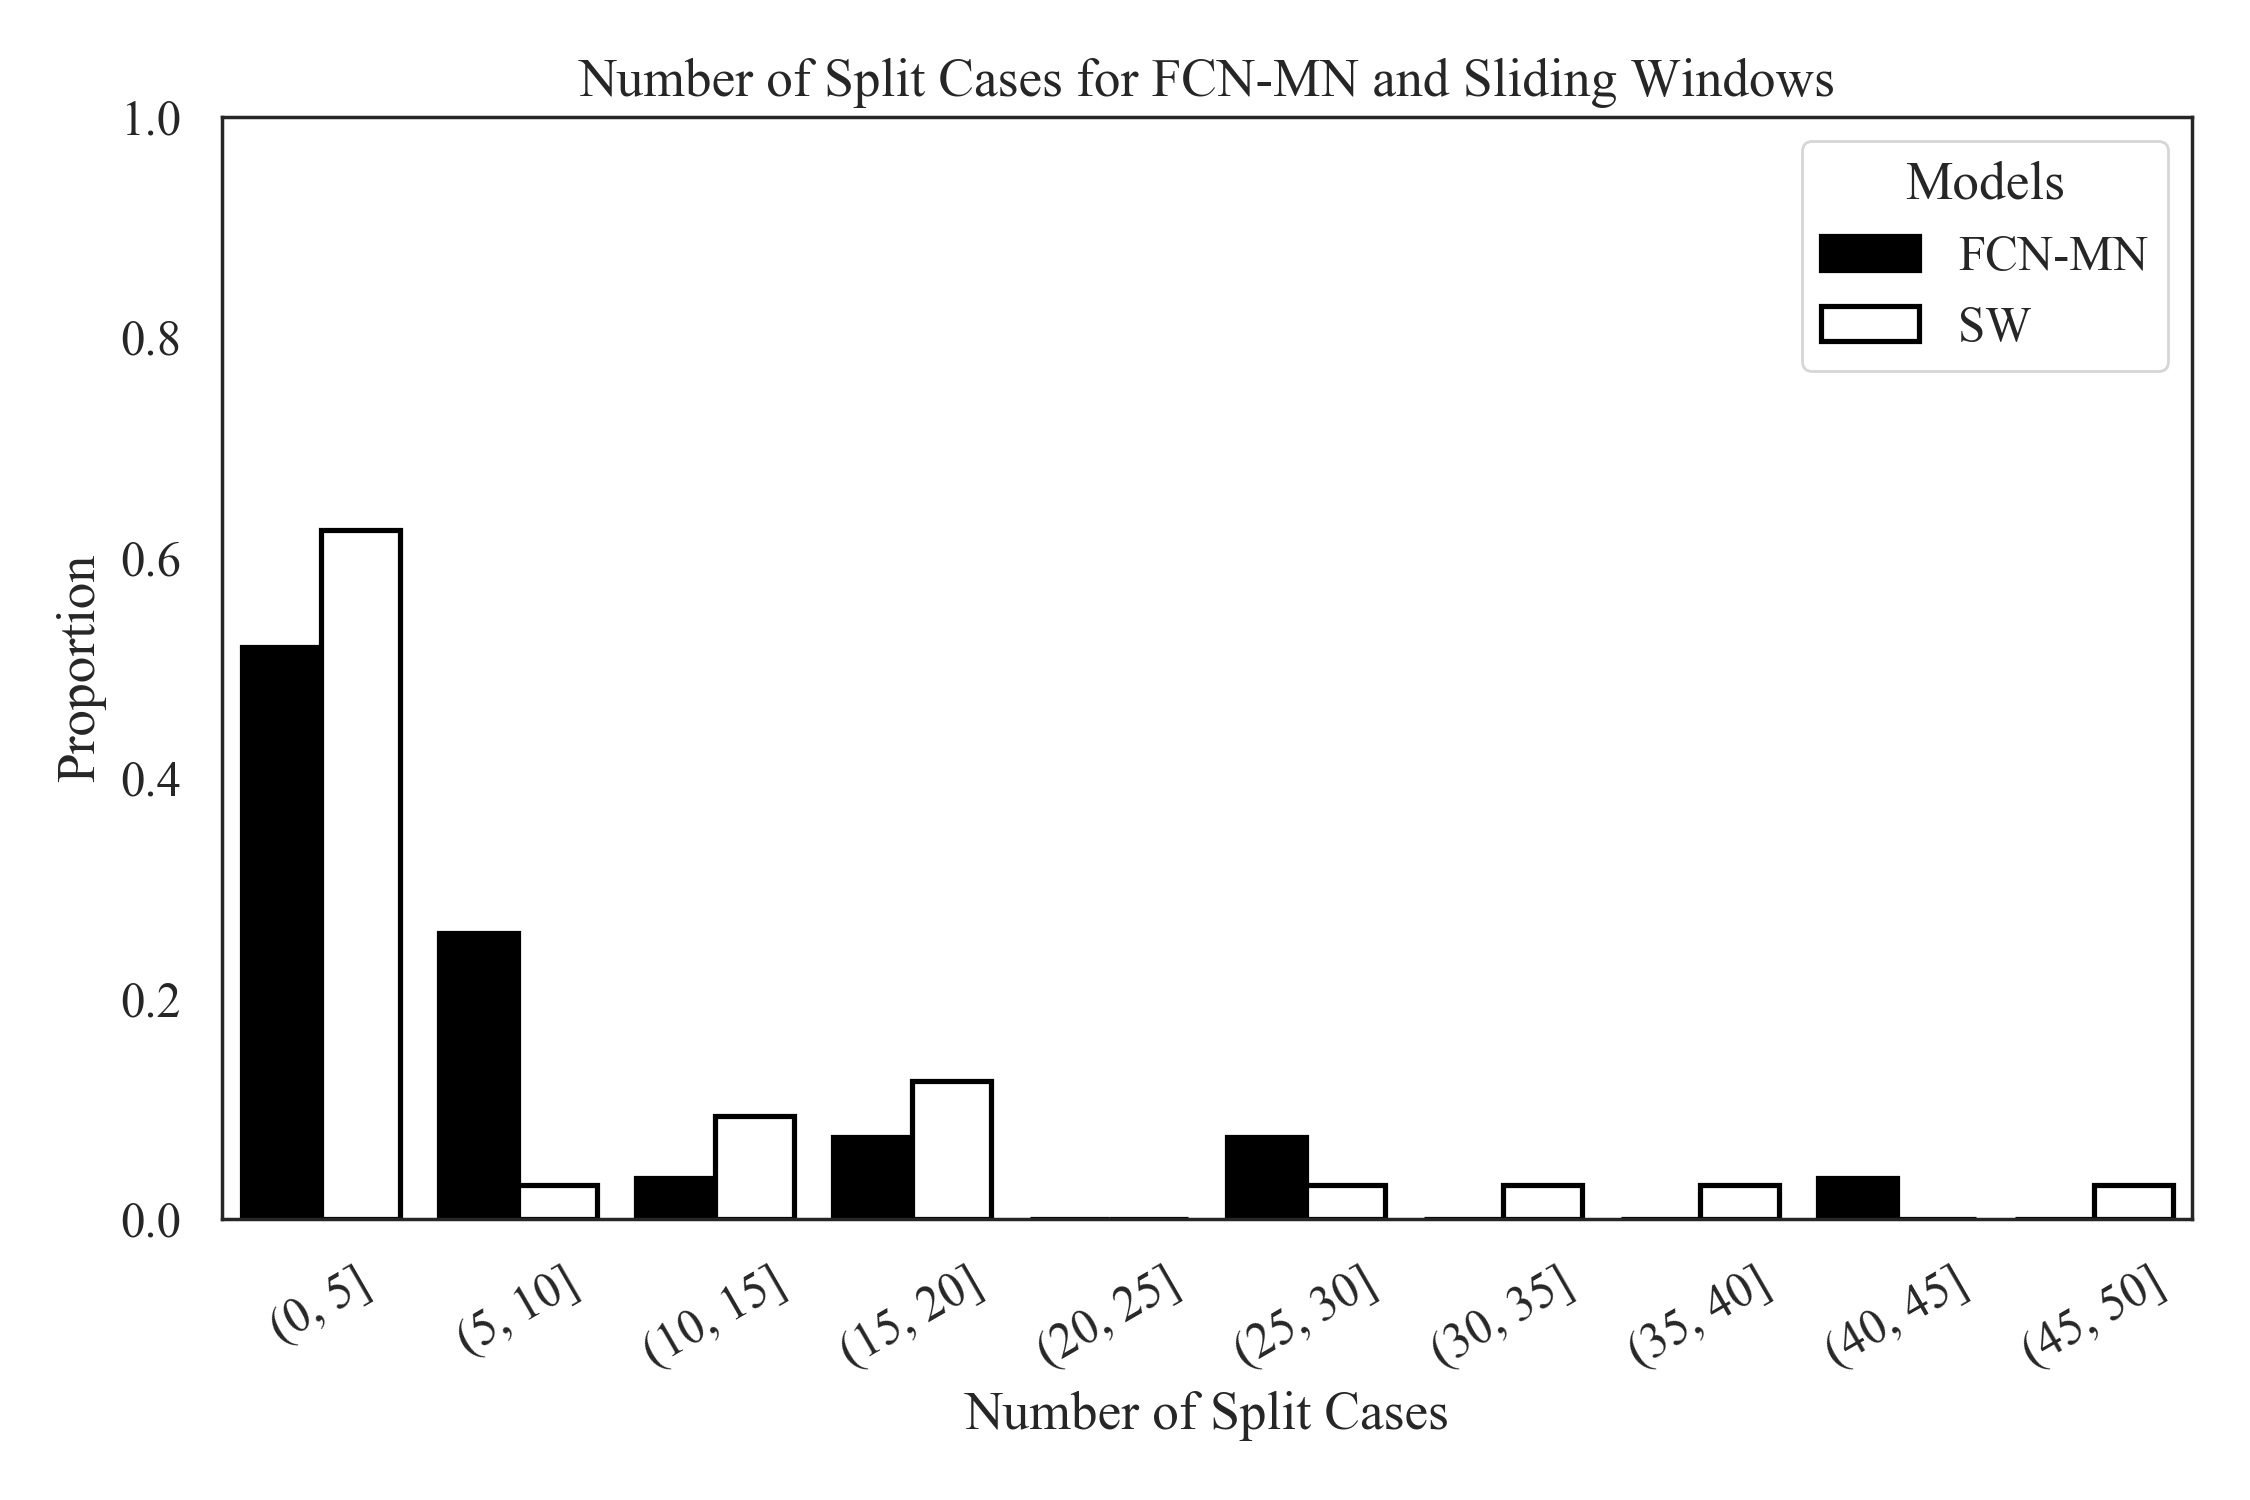
\includegraphics[width=\textwidth]{figures/PPP_split_distribution.png}
	\caption{Histogram reporting the distribution of $S$ for FCN-MN and SW in black and white bars, respectively. Each bar represents the proportion among all models ($27$ for FCN-MN  and $40$ for SW) that contains the number of splits indicated by the bin’s label. For instance, the first (from left to right) white bar indicates that almost $14\%$ out of the $40$ SW models contains between $0$ to $5$ splits. }
	\label{fig:number-of-split}
\end{figure}

\subsubsection{Detailed analysis of segmentation metrics}

As for the individualization metrics, we show in Figures \ref{fig:XXX-a} and \ref{fig:XXX-b} scatter plots for the segmentation precision and segmentation-recall, for the \emph{correct detections} and \emph{splits} cases, respectively. These correspond to their respective columns of (a non-summarized version of) Table~\ref{tab:TablaXX}, with the black and white dots representing the values of FCN-MN and SW detection models, respectively. The position of each dot in the plot corresponds to the mean segmentation-precision and mean segmentation-recall over all images in the test set, computed over the correctly detected components (splitted components, respectively) of the masks produced by the detection model associated to that dot. The standard deviation of the recall (precision) is shown as a horizontal (vertical) bar.
%
In Figure \ref{fig:XXX-a} (correctly detected), one can observe that all black dots (FCN-MN) are clustered on the upper-right corner of the graph, enclosed by a minimum precision of approximately $0.65$ and minimum recall of approximately $0.60$; while the white dots (SW) are clustered on the lower-right corner of the graph, with maximum precisions of $0.5$ and recall ranging from approximately $0.35$ to $1.0$. Overall, both algorithms show relatively high recalls, but with FCN-MN reaching much larger precisions. We can point to the coarse detection of the SW method as the main cause for the low precision, as this is reduced when extra, false positives are present in the positive mask. 
%
In Figure \ref{fig:XXX-b} (splits), one can observe again the overwhelming improvements of FCN-MN over SW, with all (but one) SW cases presenting precisions under $60\%$, with the outlier showing a precision of nearly  $70\%$, and a similar distribution of recall values.  

\begin{figure}%
	\centering
	\begin{subfigure}[b]{0.45\textwidth}
		\centering
		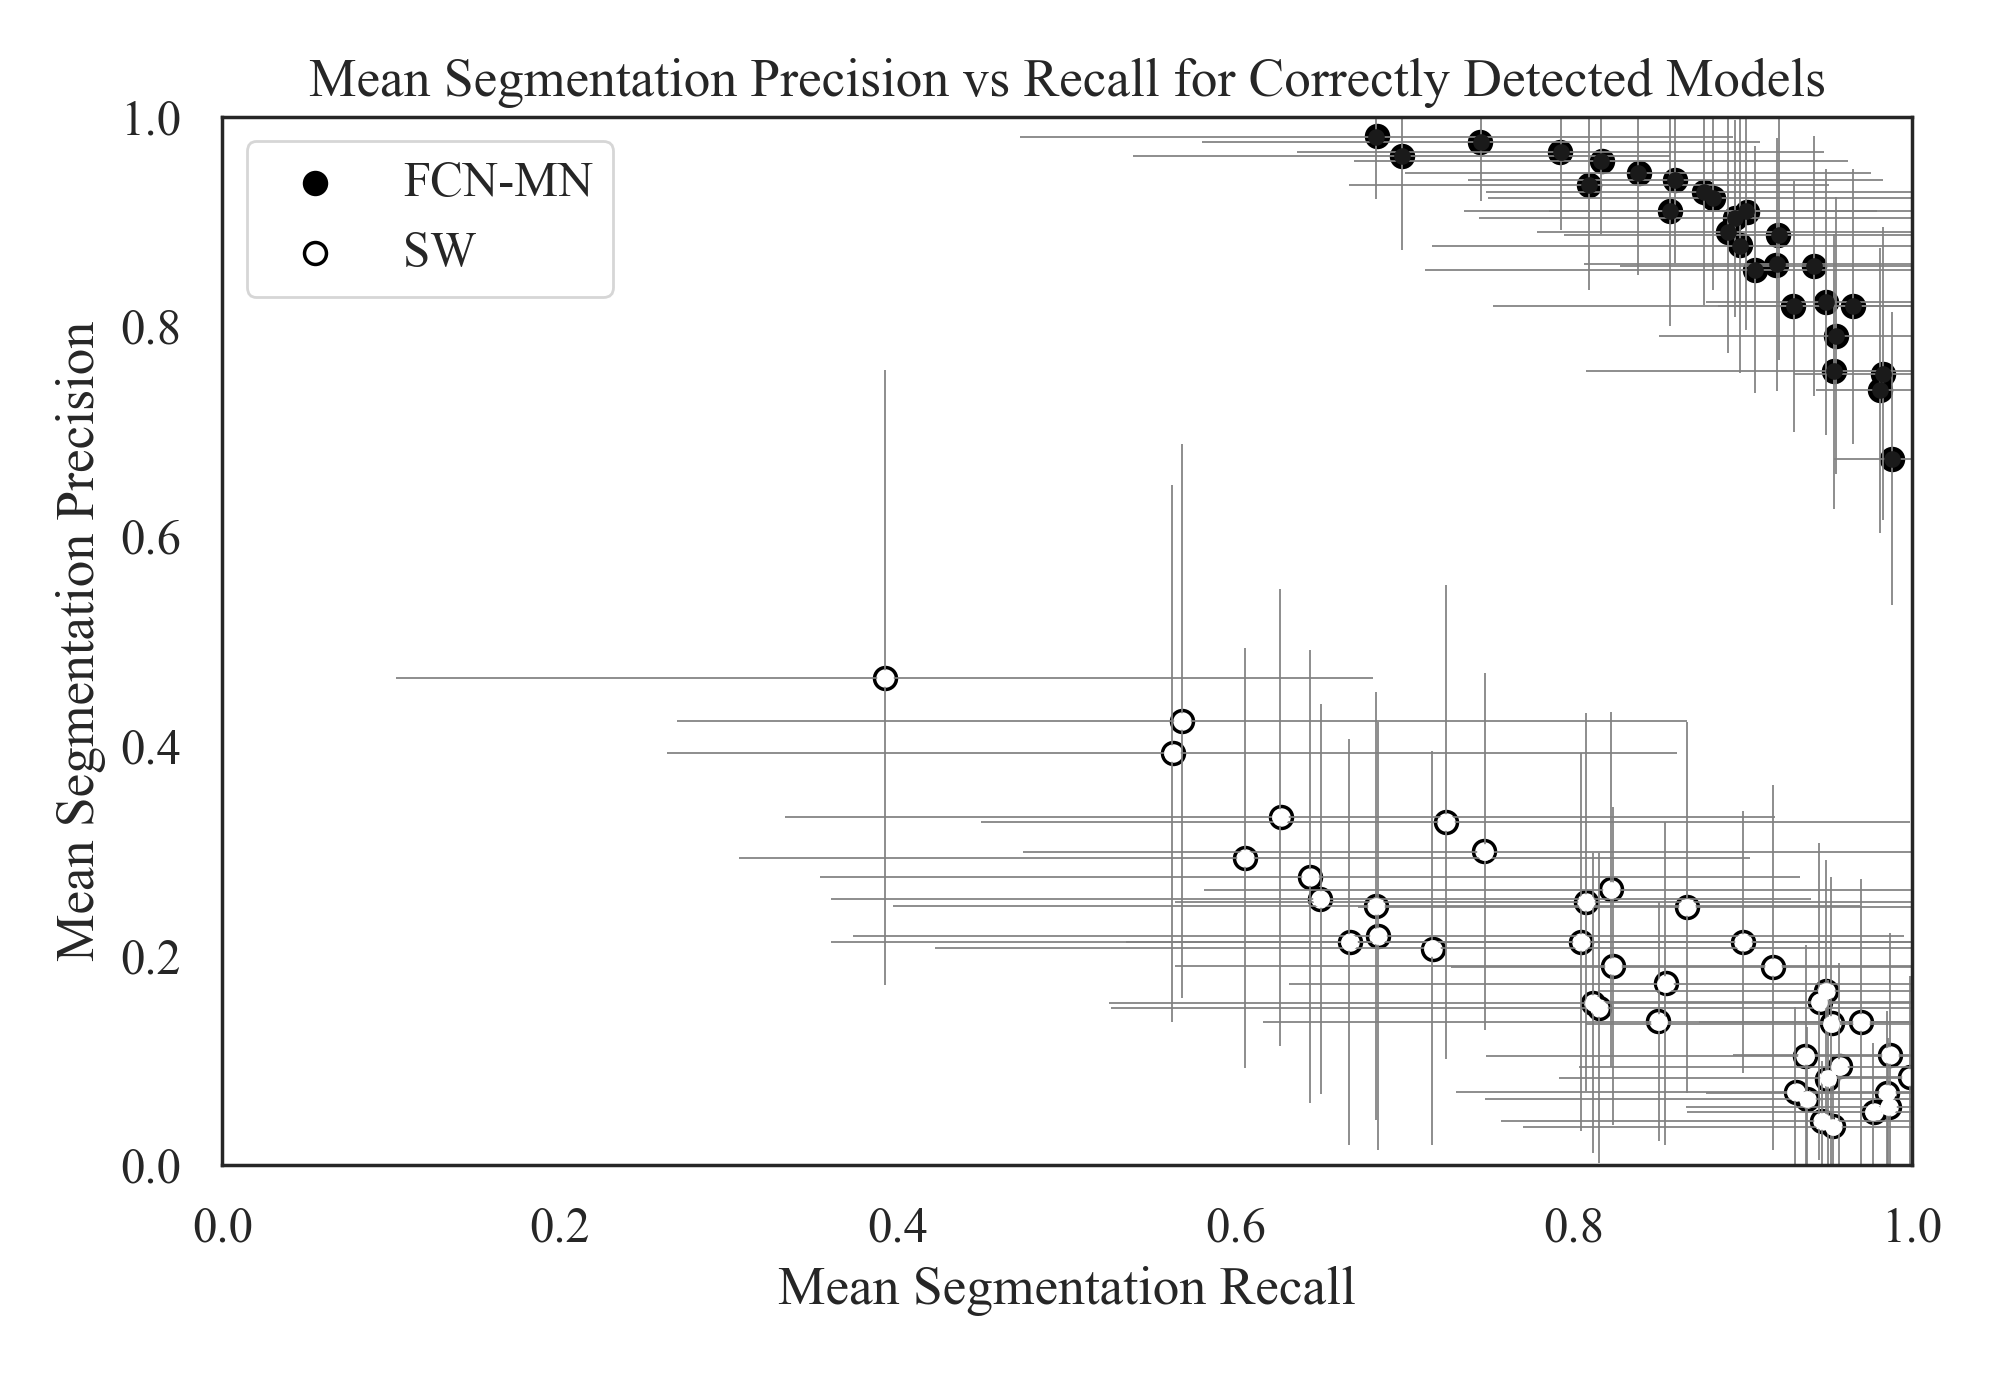
\includegraphics[width=\textwidth]{figures/XXX_correctly_detected.png}
		\caption{}
		\label{fig:XXX-a}
	\end{subfigure}
	\hfill
	\begin{subfigure}[b]{0.45\textwidth}
		\centering
		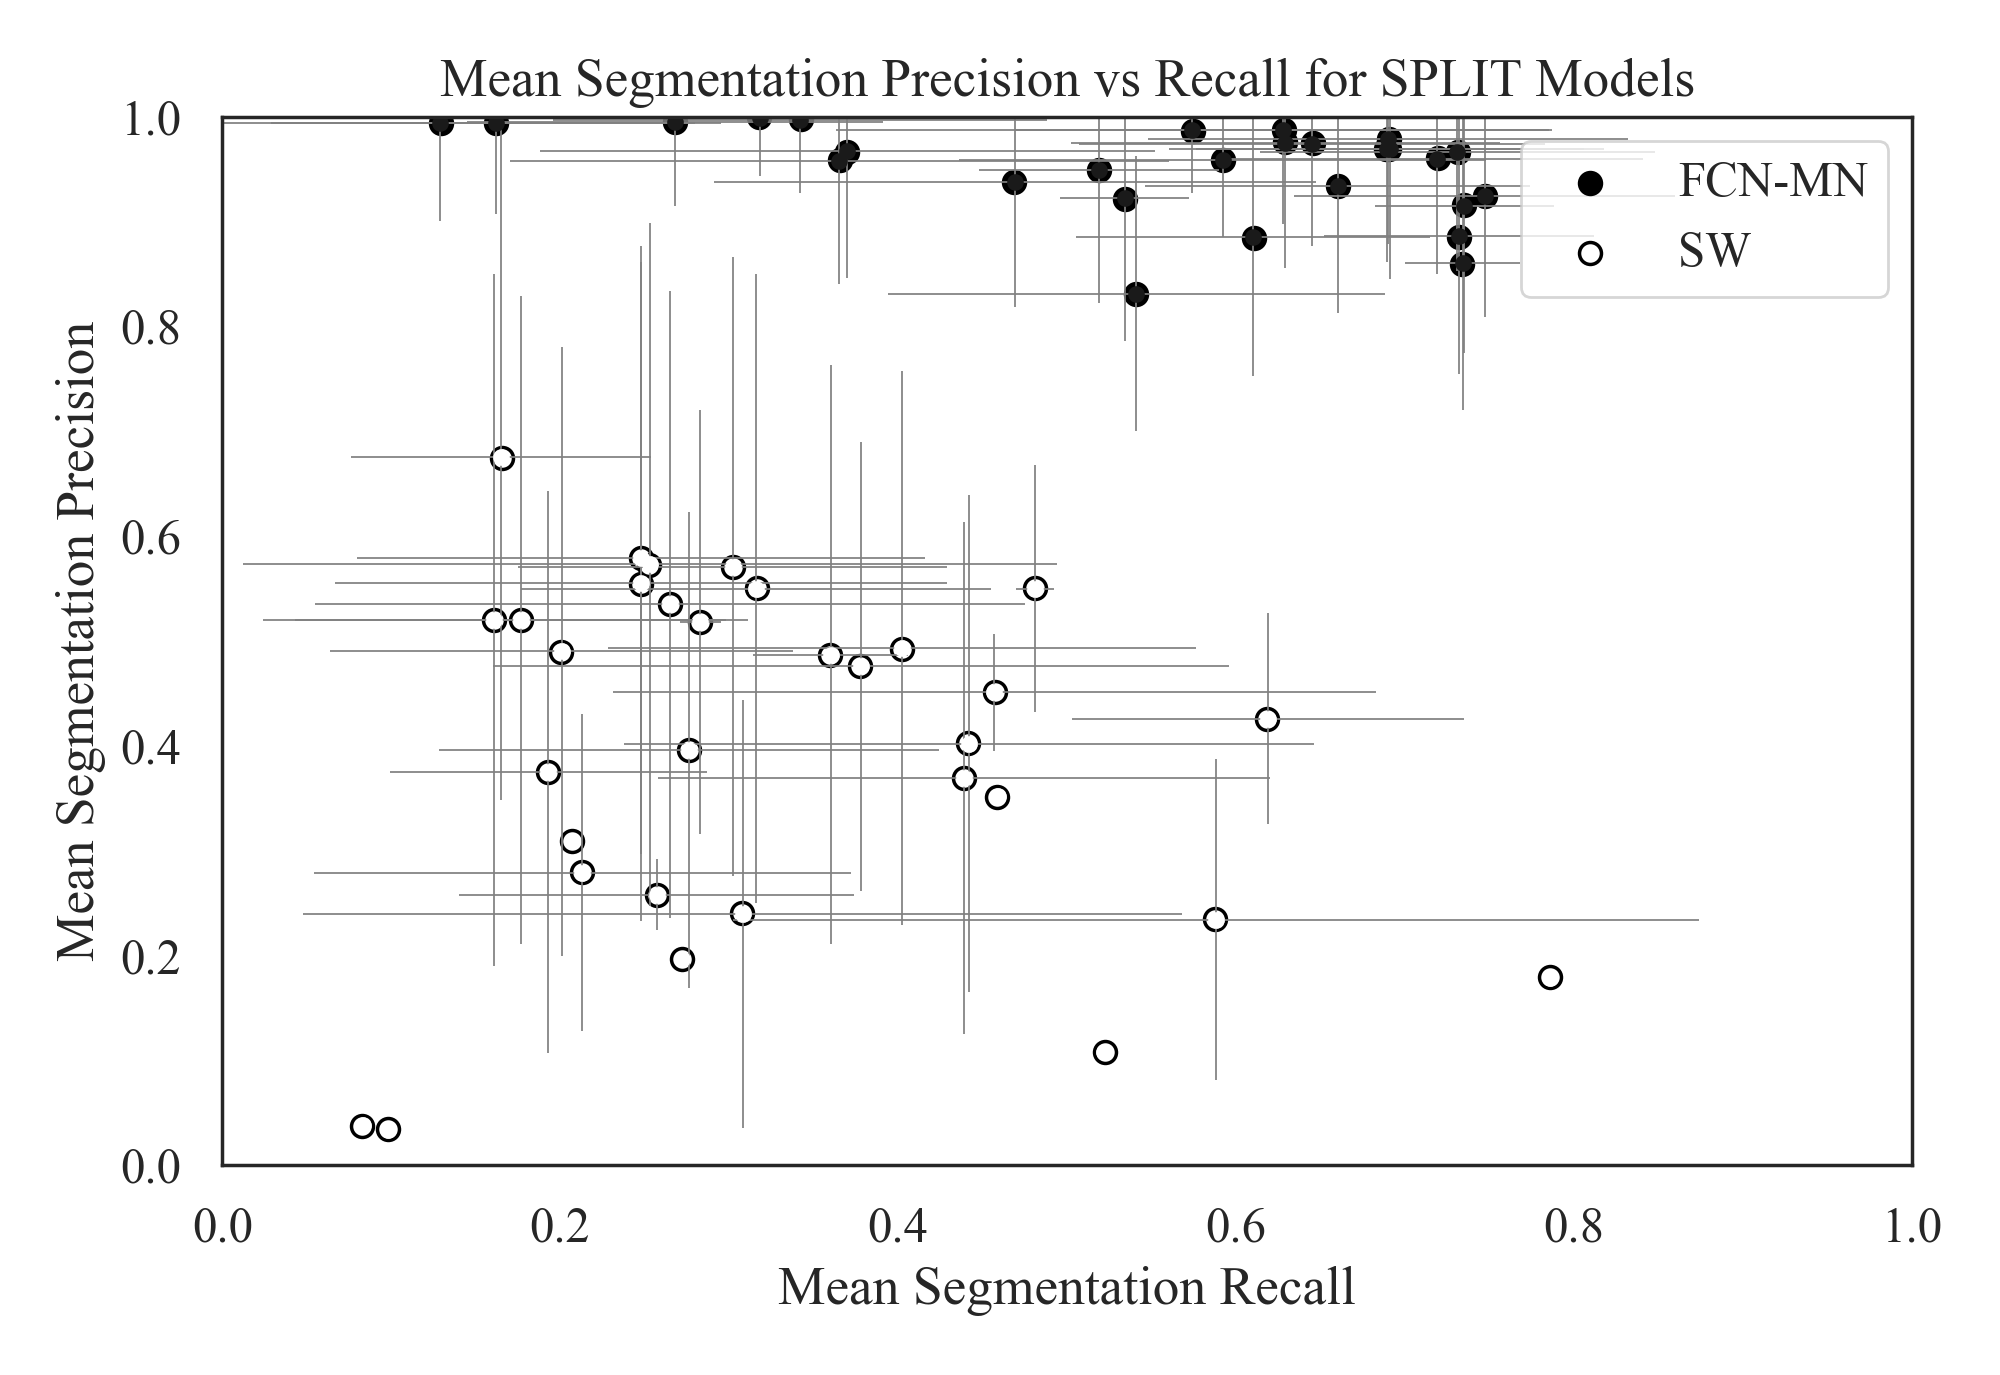
\includegraphics[width=\textwidth]{figures/XXX_splits.png}
		\caption{}
		\label{fig:XXX-b}
	\end{subfigure}
	\caption{Segmentation Precision-Recall scatterplots reporting the results for FCN-MN and SW in black and white, respectively, with dots representing the average of segmentation precision and segmentation recall over all images in the test set (and bars representing standard deviations), with one dot per configuration of hyperparameters ($27$ for FCN-MN  and $40$ for SW). In (a), the averages were computed over the segmentation precision and recall of the correctly detected components, while in (b), the averages were computed  over the segmentation precision and recall of the split components.   Standar deviations.}%
	\label{fig:XXX}%
\end{figure}

In the above results, the mean values of segmentation metrics, over all images, difflicuting any possible understanding on what happens individually for each image/bud. We thus complement the above with reports of these metrics but for individual images. For that, we selected two models/configurations for FCN-MN and two models/configurations for SW, one with the best detection F1-measure  and one with the best Dice metric (i.e., segmentation F1-measure). The selected detection models are FCN-MN$_{16s}^{0.6}$,  FCN-MN$_{16s}^{0.8}$, SW$_{1000}^{1}$, and SW$_{100}^{3}$. 
%
As above, we discriminate the results for the \emph{correctly detected} and \emph{splitted} components, shown in Figures \ref{fig:ZZZ-a} and \ref{fig:ZZZ-b},  respectively. These figures show four scatterplots each, one for each of the four cases, with black squares for FCN-MN$_{16s}^{0.6}$, black circles for  FCN-MN$_{16s}^{0.8}$, white squares for SW$_{1000}^{1}$, and white circles for SW$_{100}^{3}$.  Here, the position of each point in the scatter plot is representing the segmentation-precision and segmentation-recall of the one correctly detected of one single image (Figure \ref{fig:ZZZ-a}), and the joint splits of one single image (Figure \ref{fig:ZZZ-b})
%
These figures show the same trend shown for the plots over detection models, where FCN-MN (black squares and circles) overwhelmingly improves over SW (white squares and circles). For the correctly detected (Figure \ref{fig:ZZZ-a}),  one can see an even more pronounced clustering of FCN-MN (black) dots on the upper-right corner with precisions much higher than those of SW (white), with some outliers of small recall, or small precision; clearly those responsible for lowering the mean precision and recall reported in the table and figures above. Also, one can observe two different behaviours for the white dots (SW), where both present recall values over the whole range, but the white circles (SW with highest Dice) show considerably higher precisions, with some cases over $0.6$.  
%
The split case, Fig. \ref{fig:ZZZ-b},  shows some interesting conclusions as well. First we note that the case of SW with window size of 1000px (white circle) has no points in the scatter plot, as a result of no splits for that case. This is expected given the large size of the patch. Also, one can notice that all split components of both cases of FCN-MN (black squares and black circles)  have precision of practically $1.0$, while the (single) case of SW presents several split components with small precision. Large precision, regardless of the recall, shows these splits are correct detection that has been splitted, that is, components that are entirely within the true bud but that are not connected among themselves. 

\begin{figure}%
	\centering
	\begin{subfigure}[b]{0.45\textwidth}
		\centering
		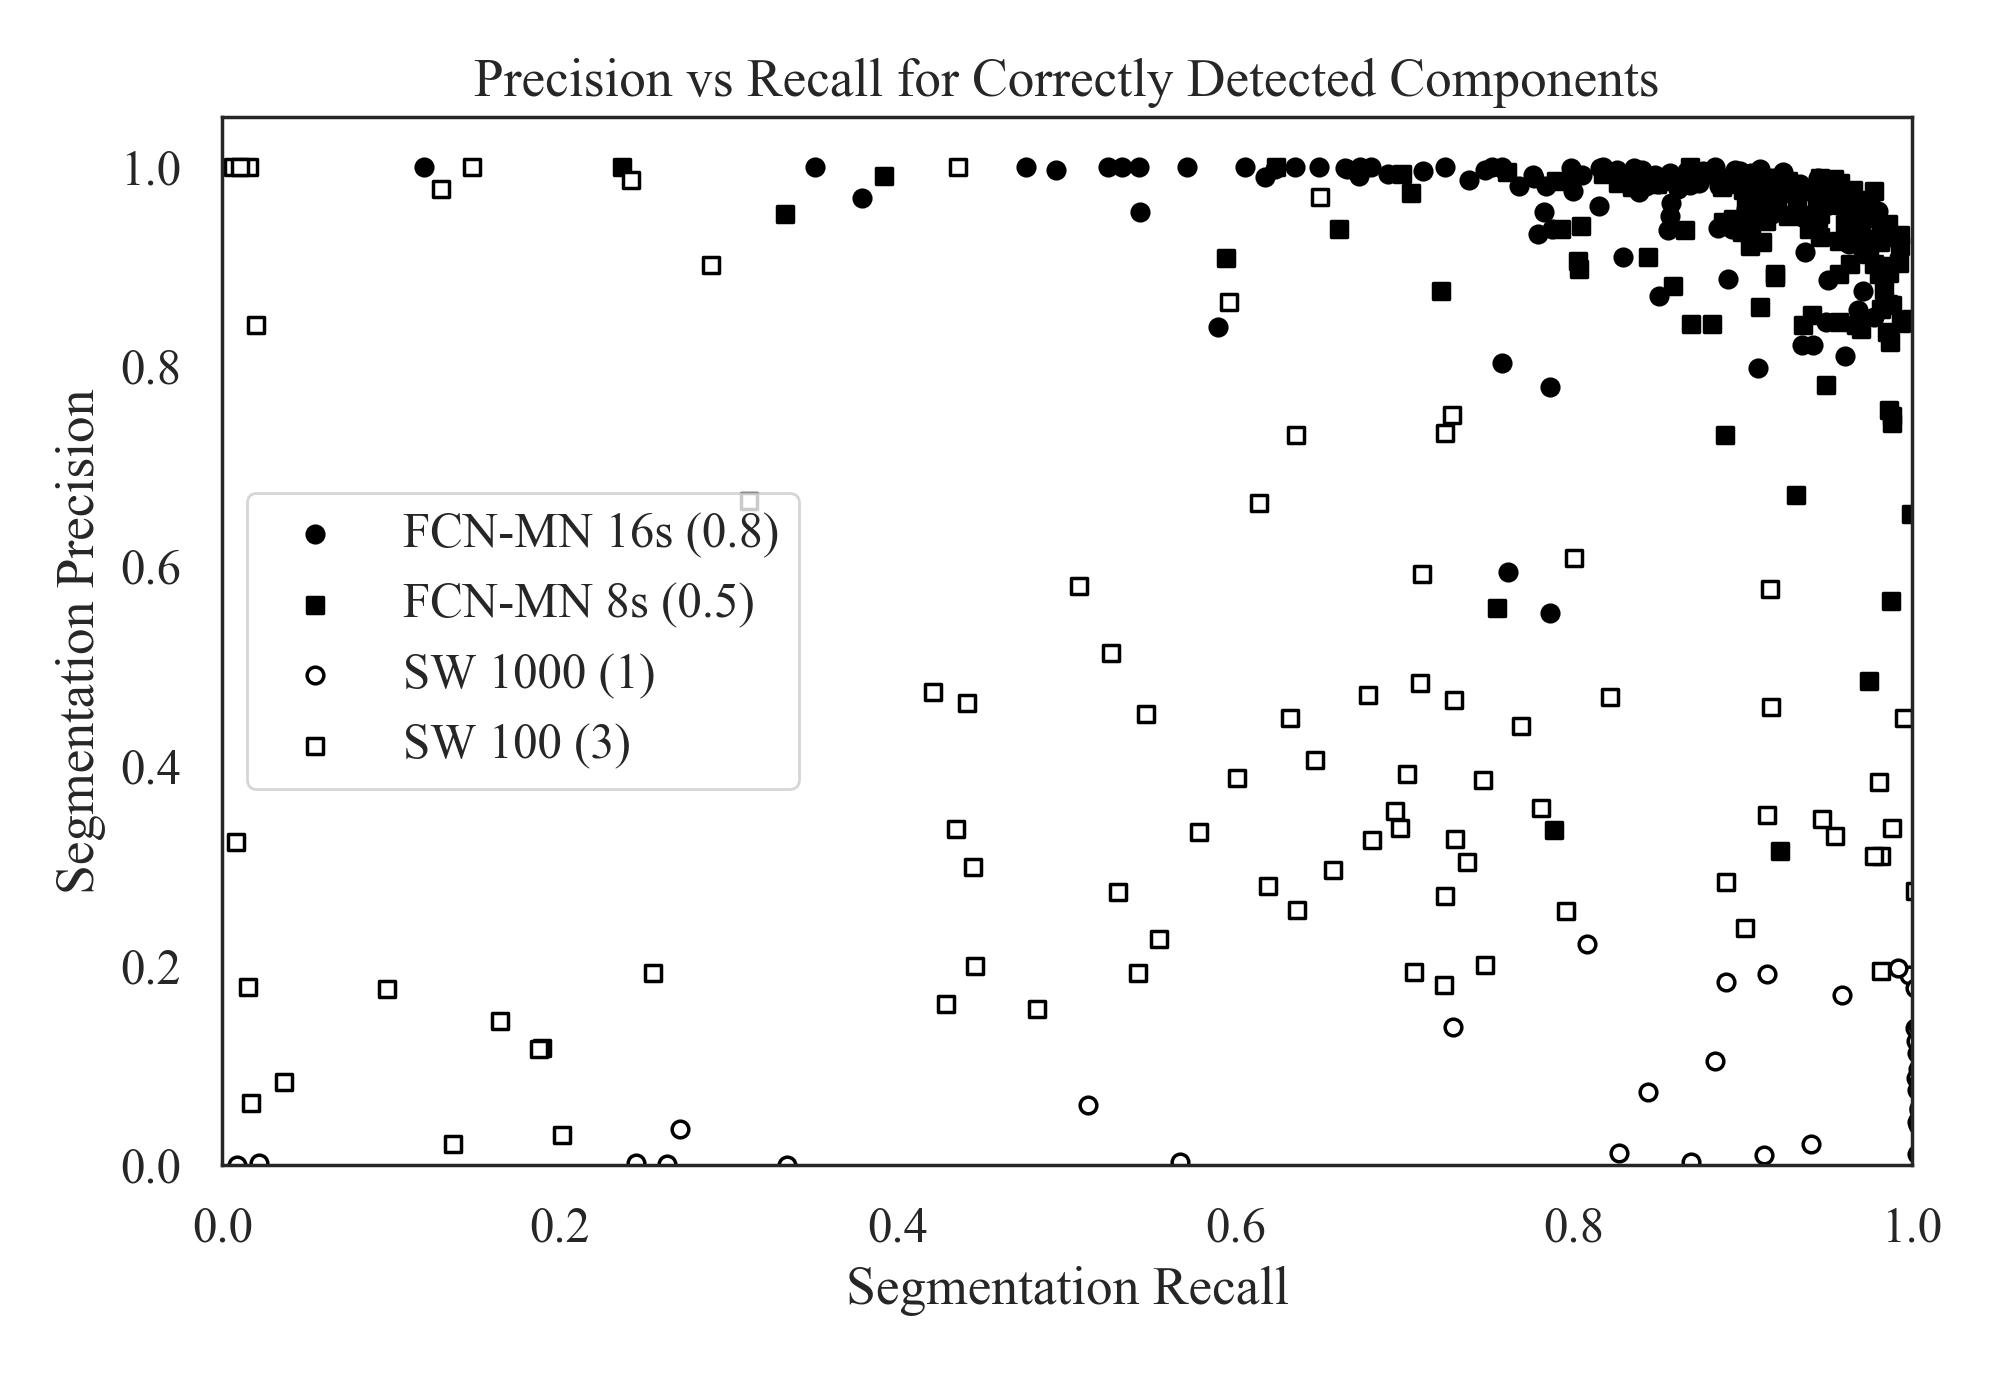
\includegraphics[width=\textwidth]{figures/ZZZ_correctly_detected.png}
		\caption{}
		\label{fig:ZZZ-a}
	\end{subfigure}
	\hfill
	\begin{subfigure}[b]{0.45\textwidth}
		\centering
		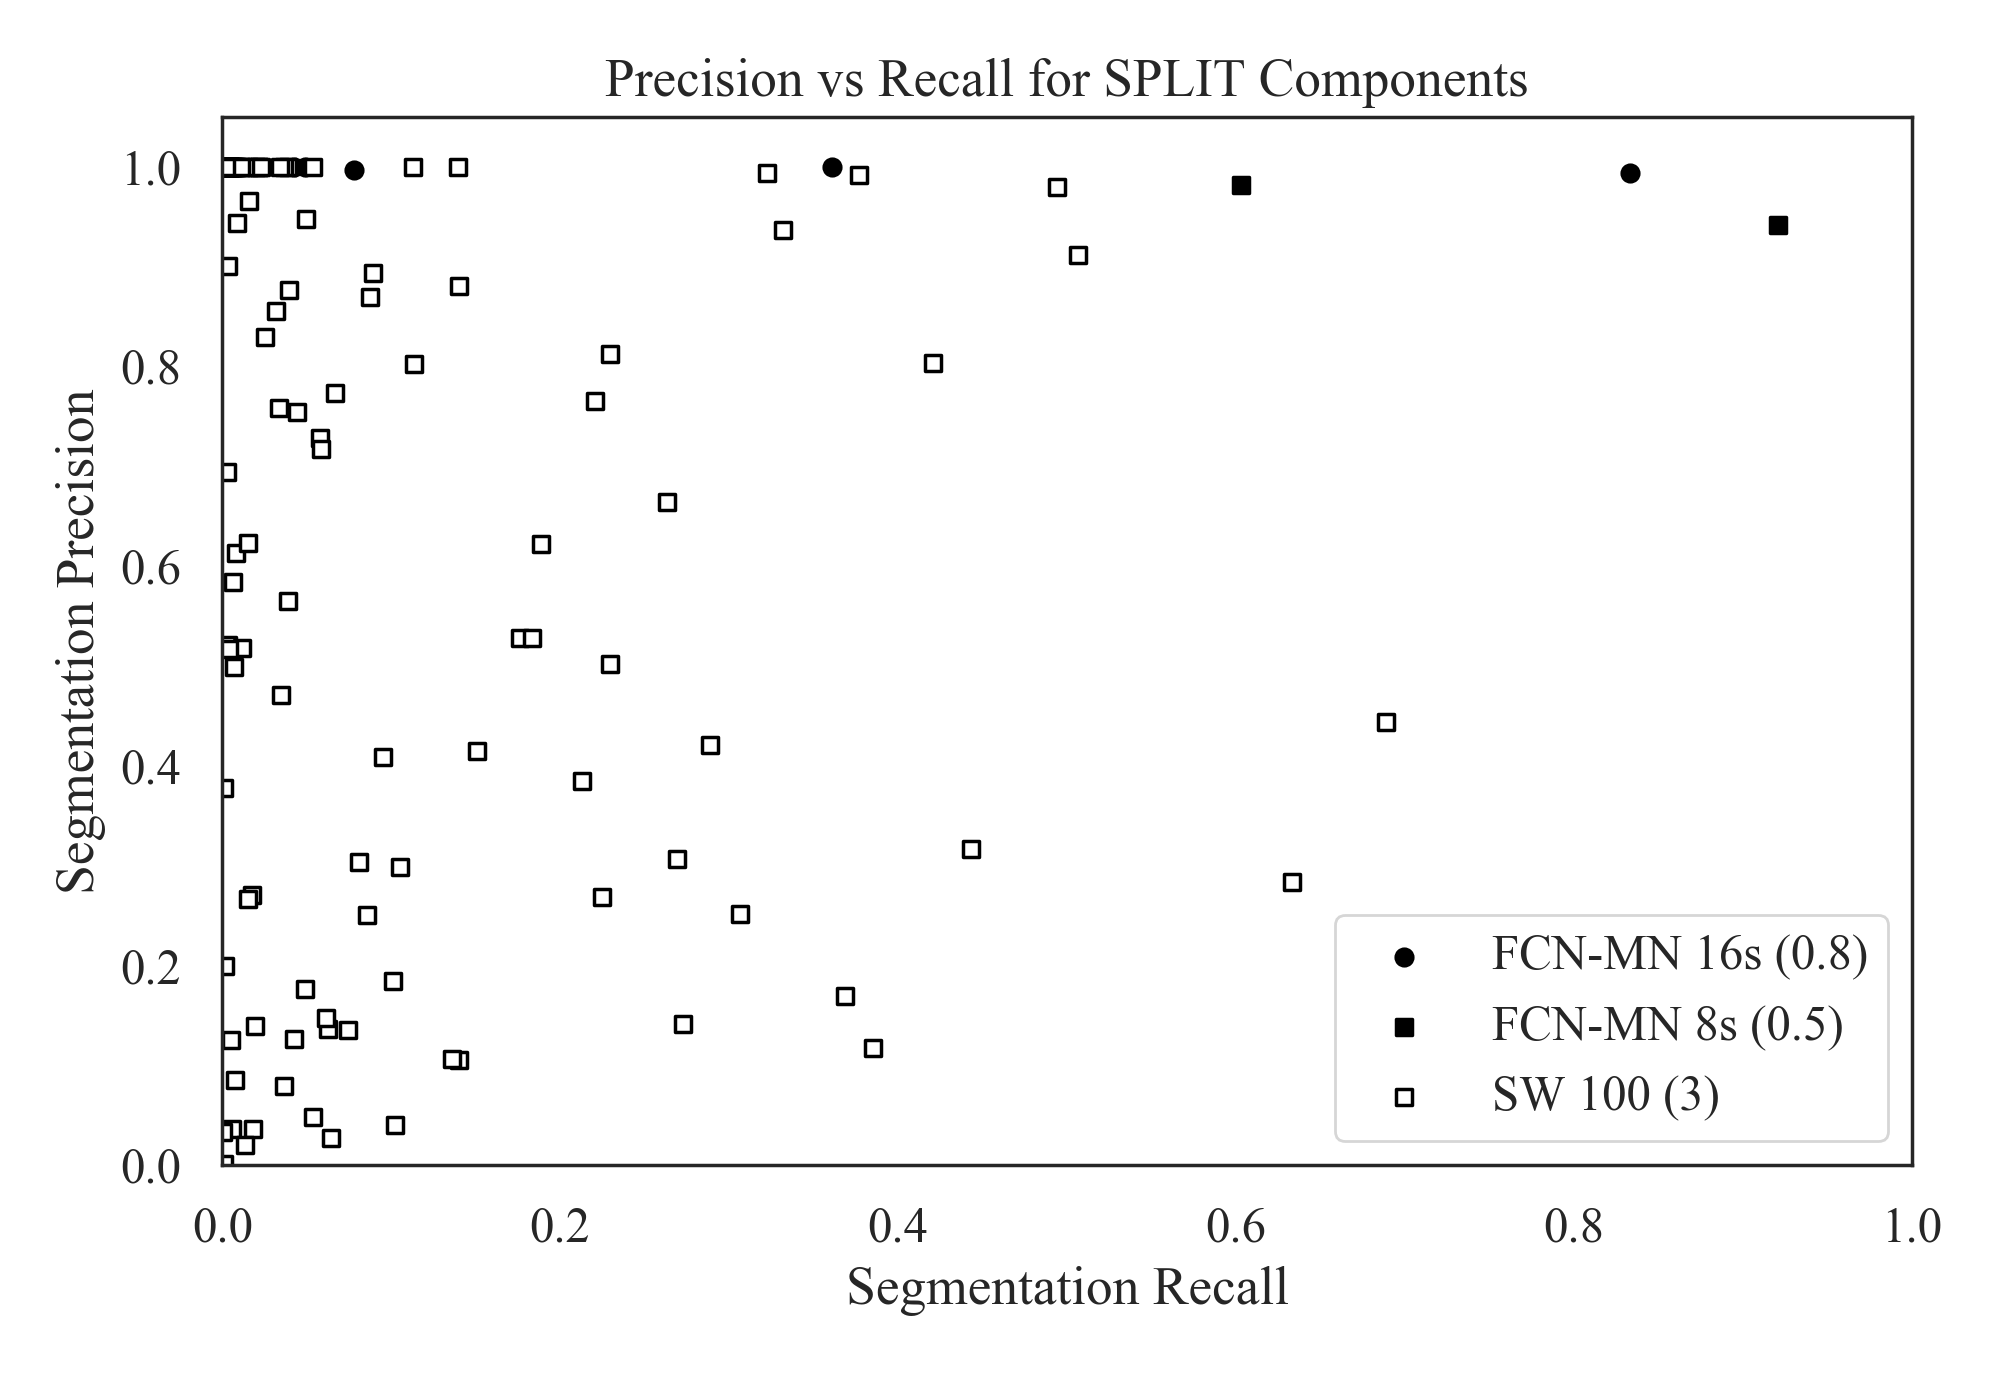
\includegraphics[width=\textwidth]{figures/ZZZ_splits.png}
		\caption{}
		\label{fig:ZZZ-b}
	\end{subfigure}
	\caption{ Segmentation precision and recall for masks of single images obtained by four detection models FCN-MN$_{16s}^{0.6}$,  FCN-MN$_{16s}^{0.8}$, SW$_{1000}^{1}$, and SW$_{100}^{3}$ with higher detection F1-measure and higher Dice measure. In  (a) only correctly detected are considered, and in (b) only splits.}%
	\label{fig:ZZZ}%
\end{figure}

%%%%%%%%%
\subsection{Reports for False Alarms} 
\label{sec:falsealarmsrep}

% Figure AAA

\begin{figure}%
	\centering
	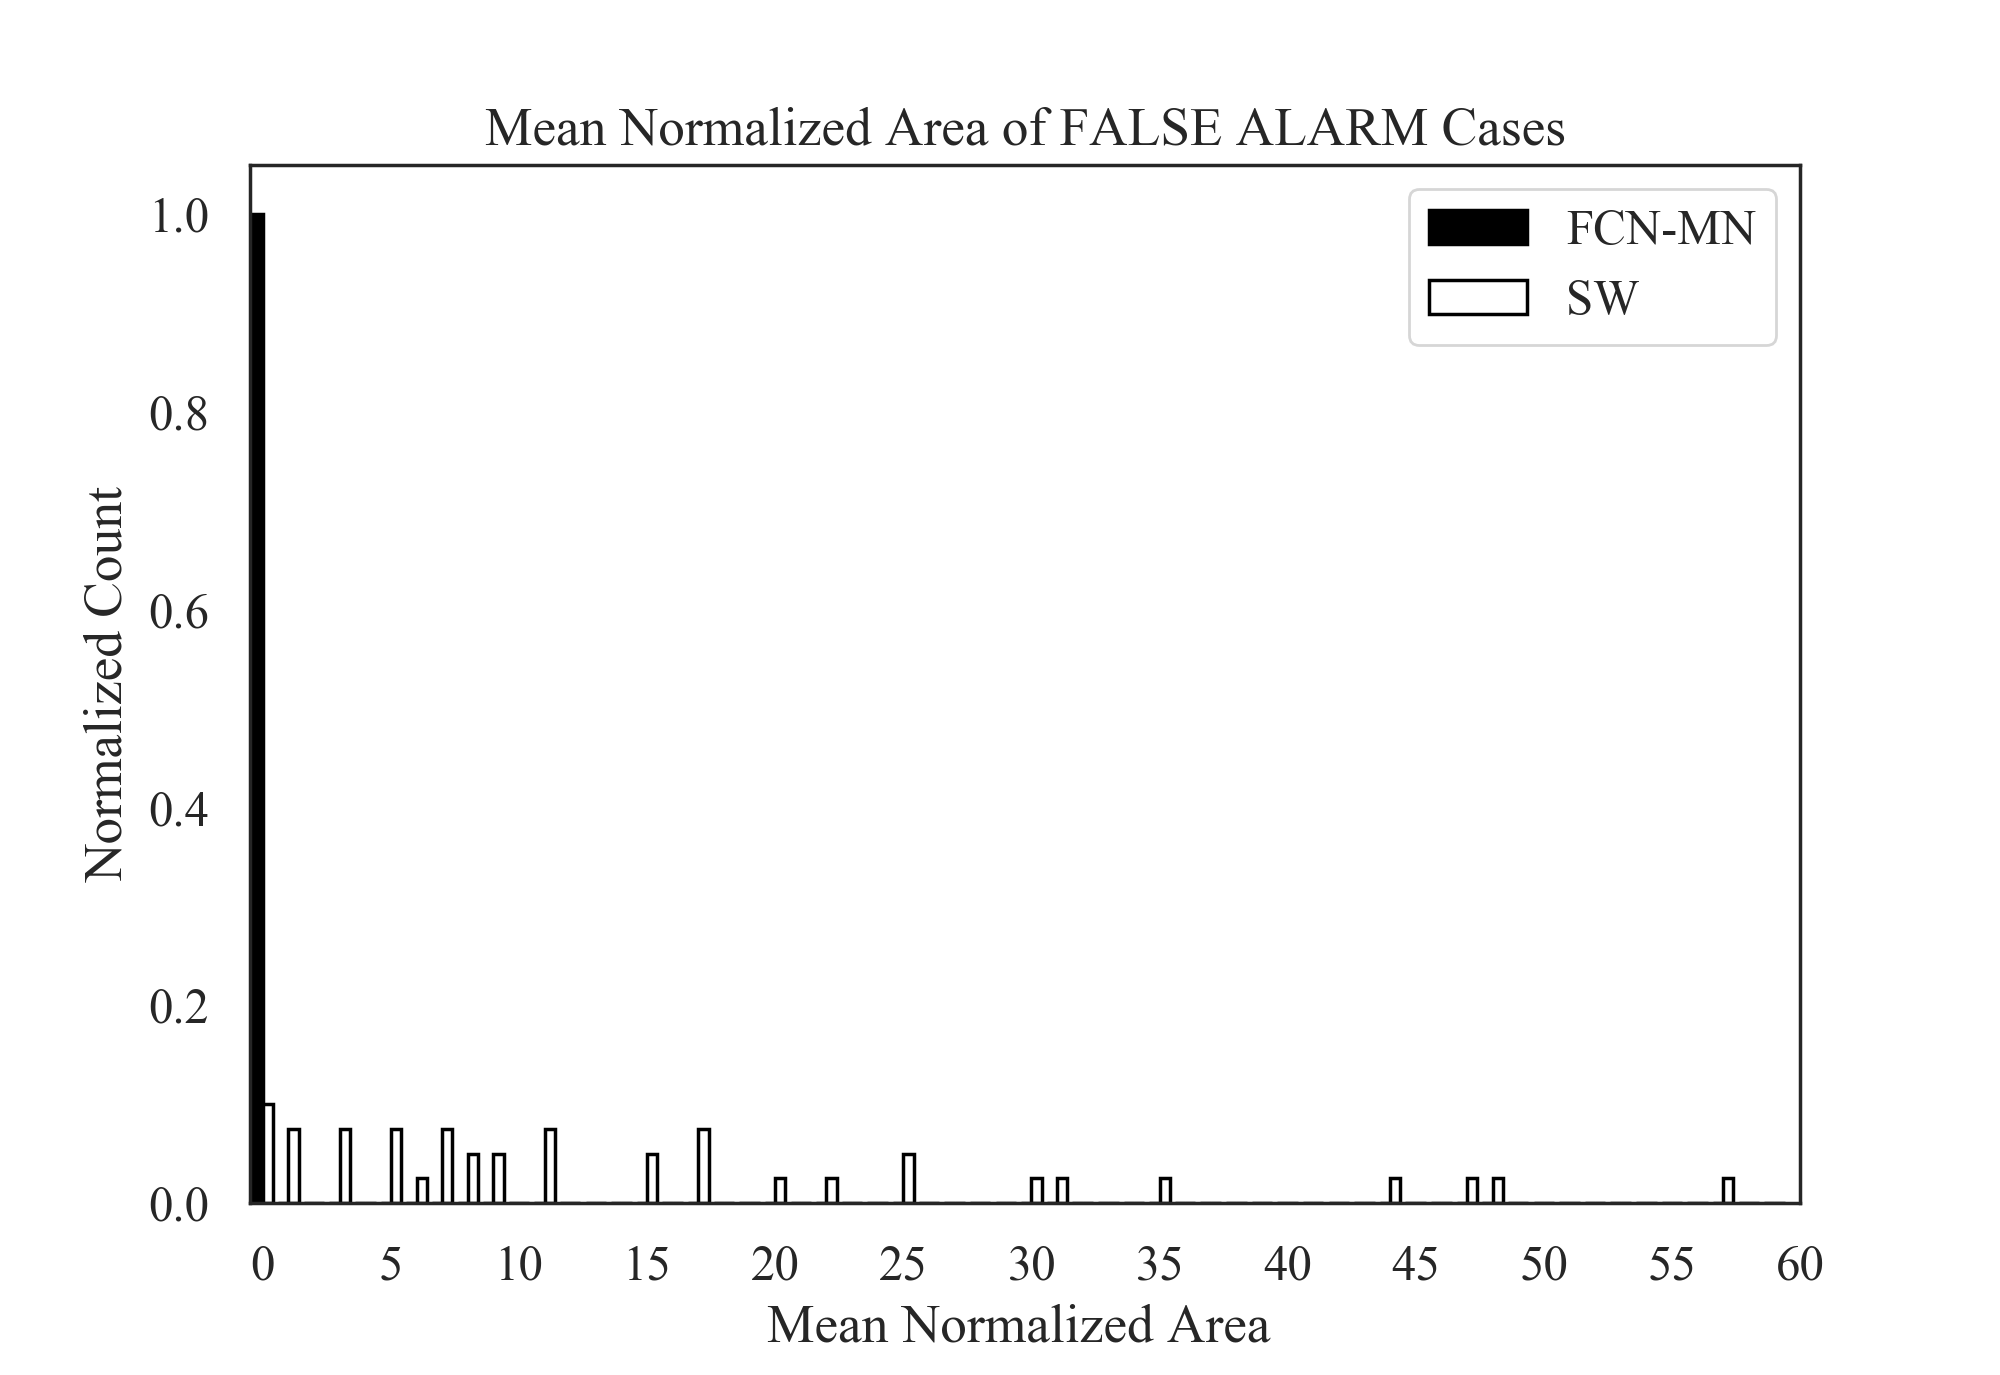
\includegraphics[width=\textwidth]{figures/AAA_mean_relative_area_fcn_vs_sw.png}%
	\caption{TODO:redactar}
	\label{fig:AAA}
\end{figure}

We also report graphically the segmentation results for the false alarm, the $NA$  for each of the $27$ models of FCN and each of the $40$ models of SW, i.e., for each cell in the  one-before-last column of (a non-summarized version of) Table~\ref{tab:TablaXX}
%
Figure~\ref{fig:AAA} shows these results grouped in the form of two histograms, one for the FCN-MN detection models (black) and one for the SW models (in white). Bars in the histogram represent the proportion of detection models whose mean $NA$ (over all all false alarm components of all images) falls within the interval of the bin. The more concentrate to the left, the better is the algorithm, as this indicates that more detection models for that algorithm resulted in smaller $NA$ (on average).
%
One can observe the histogram for FCN-MN considerably more concentrated at the left-most part of the histogram than that of SW, with all FCN-MN concentrated in a single bar at the left-most interval of  $[0.0, 1.0)$. For SW the situation is rather different, with bars at intervals as far to the right as $[57.0, 58.0)$, that is, detection models with areas as large as $58$ times the area of the bud. 
%
\begin{figure}%
	\centering
	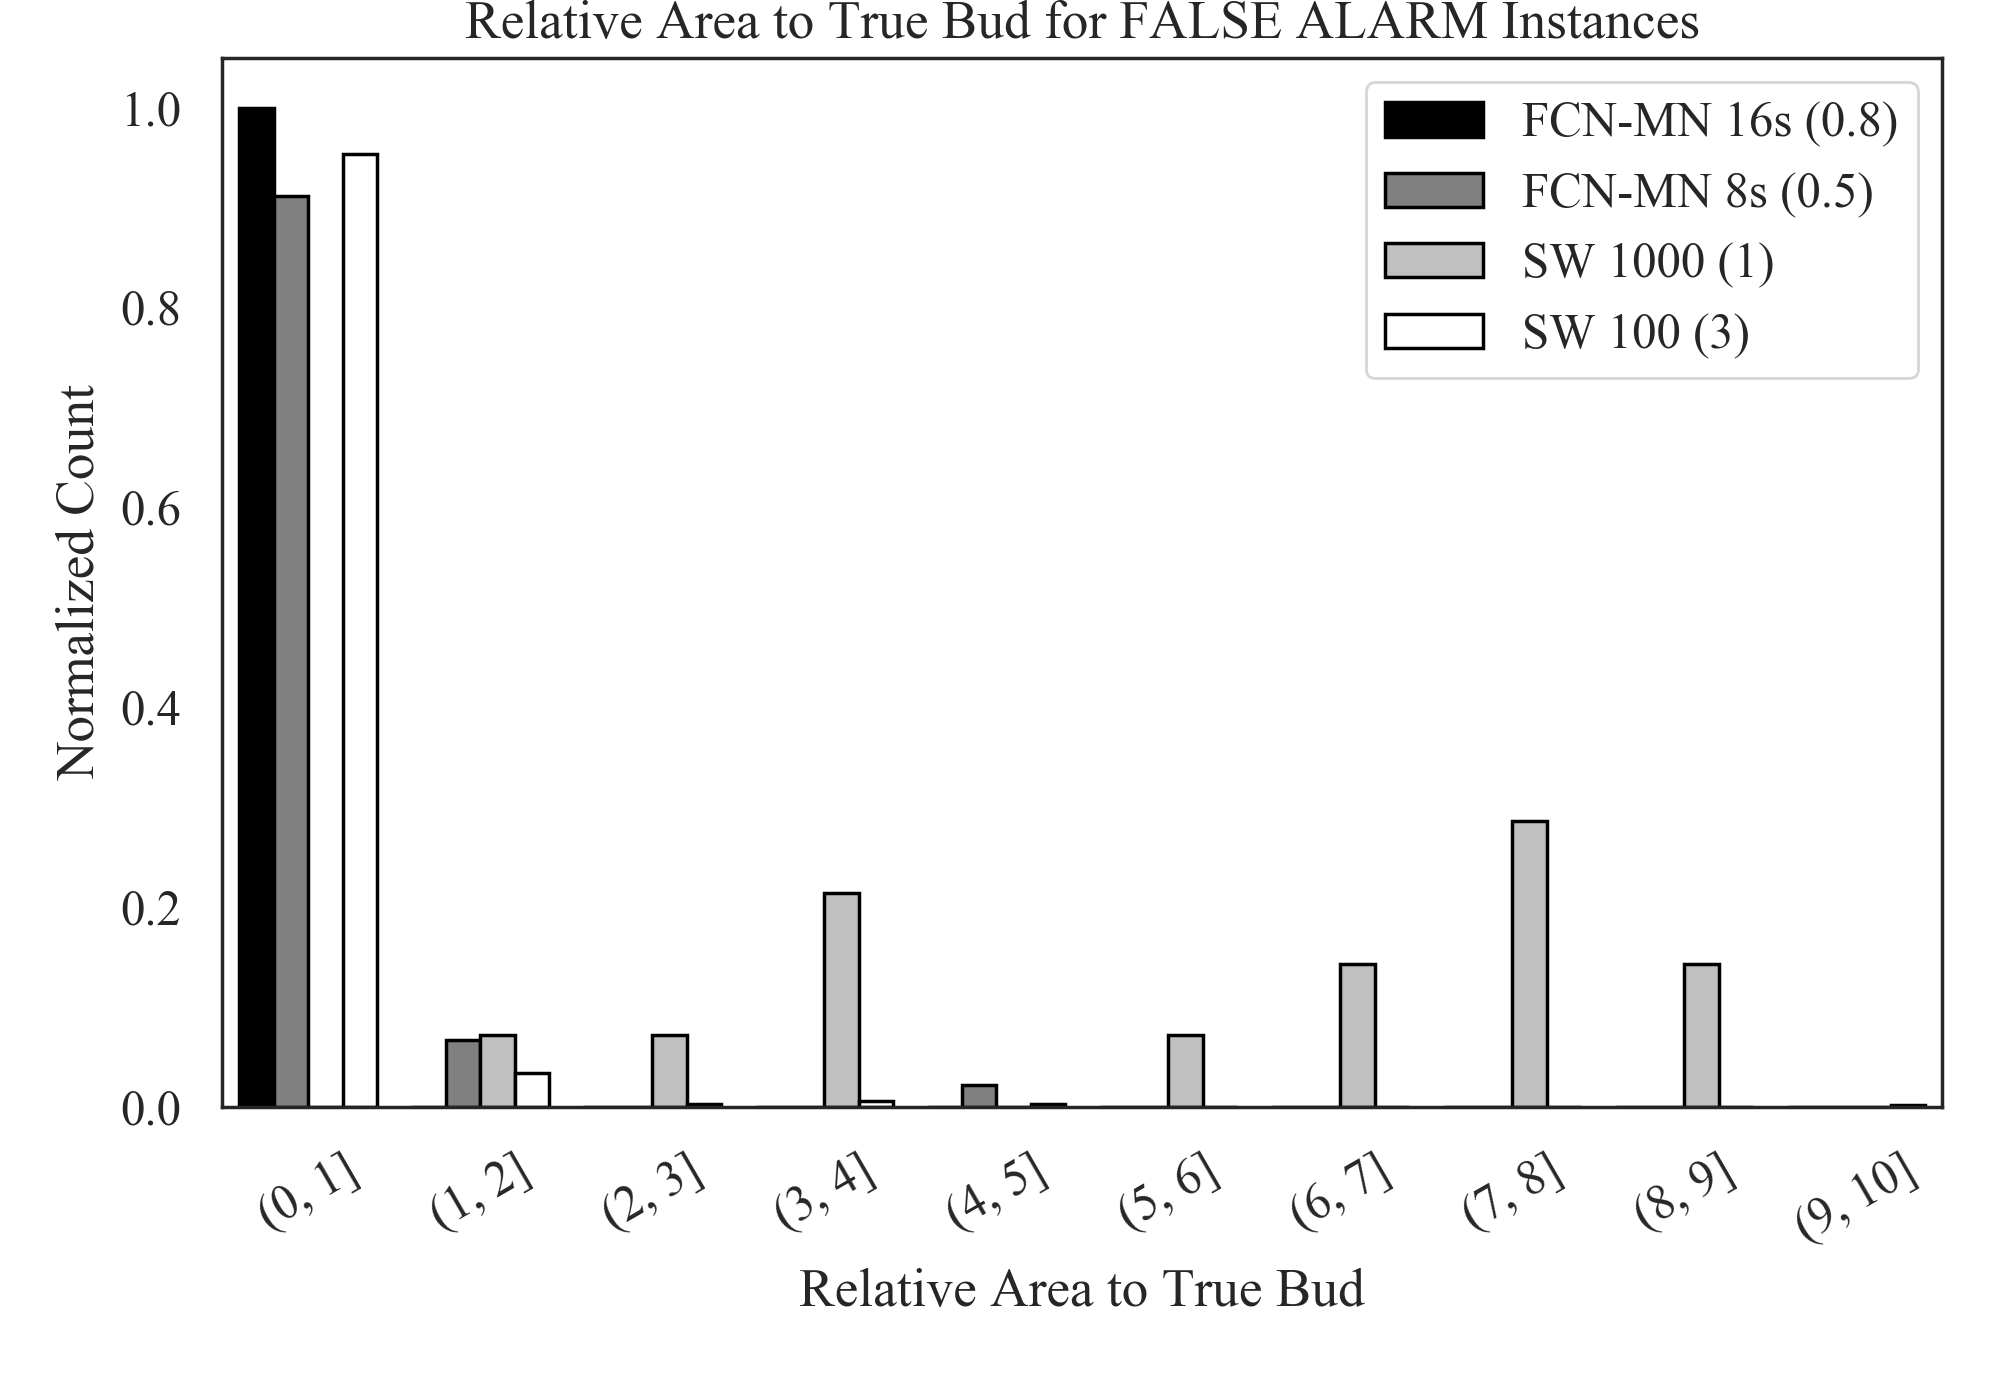
\includegraphics[width=\textwidth]{figures/CCC_relative_area_false_alarm.png}
	\caption{Figure CCC a for the normalized área (NA).}%
	\label{fig:truebud-FA-a}
\end{figure}

%%%%%%%%%%%%%%%%%%%%%%%%
\subsubsection{Detailed analysis of localization metrics}


To appreciate details on the $ND$ values of individual false alarm components we considered the same four detection models selected above for the best F1 (detection) and Dice (segmentation) measures. 
% 
Figure~\ref{fig:CCC-b} shows a histogram for $ND$ over images for the four models. Once again the advantage of FCN-MN over SW is clear, with FCN-MN producing false alarm components at a distance of at most 3-4 bud diameters (with one outlier at 7), while SW produces false alarm components at around 6 to 10 diameters of a bud.

\begin{figure}%
	\centering
	\begin{subfigure}[b]{0.45\textwidth}
		\centering
		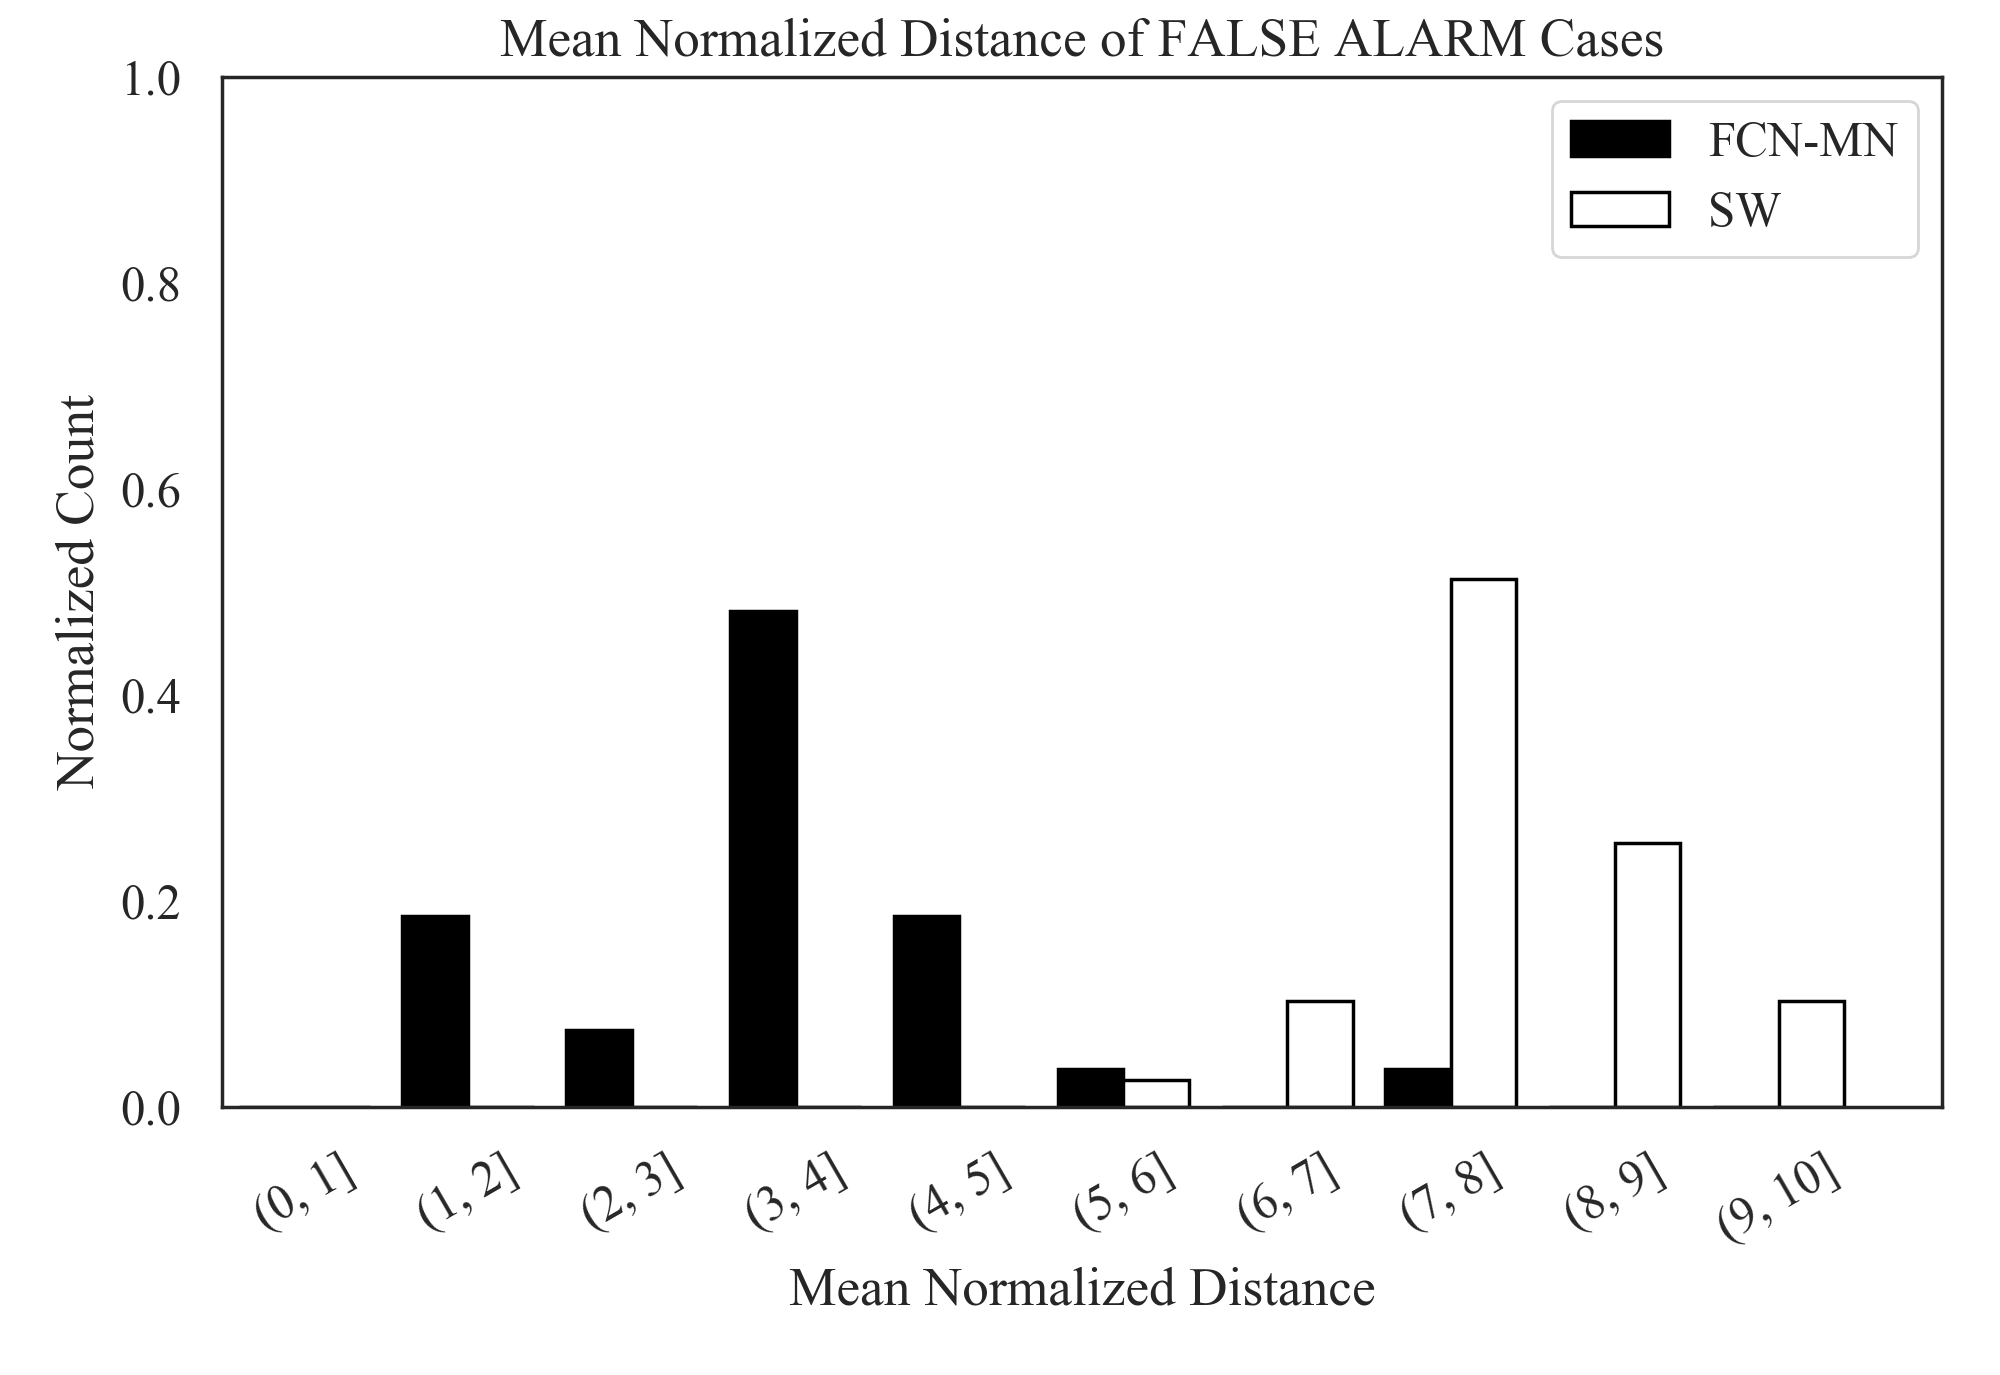
\includegraphics[width=\textwidth]{figures/AAA_normalized_distance_falsealarm_fcn_sw.png}
		\caption{}
		\label{fig:CCC-a}
	\end{subfigure}
	\hfill
	\begin{subfigure}[b]{0.45\textwidth}
		\centering
		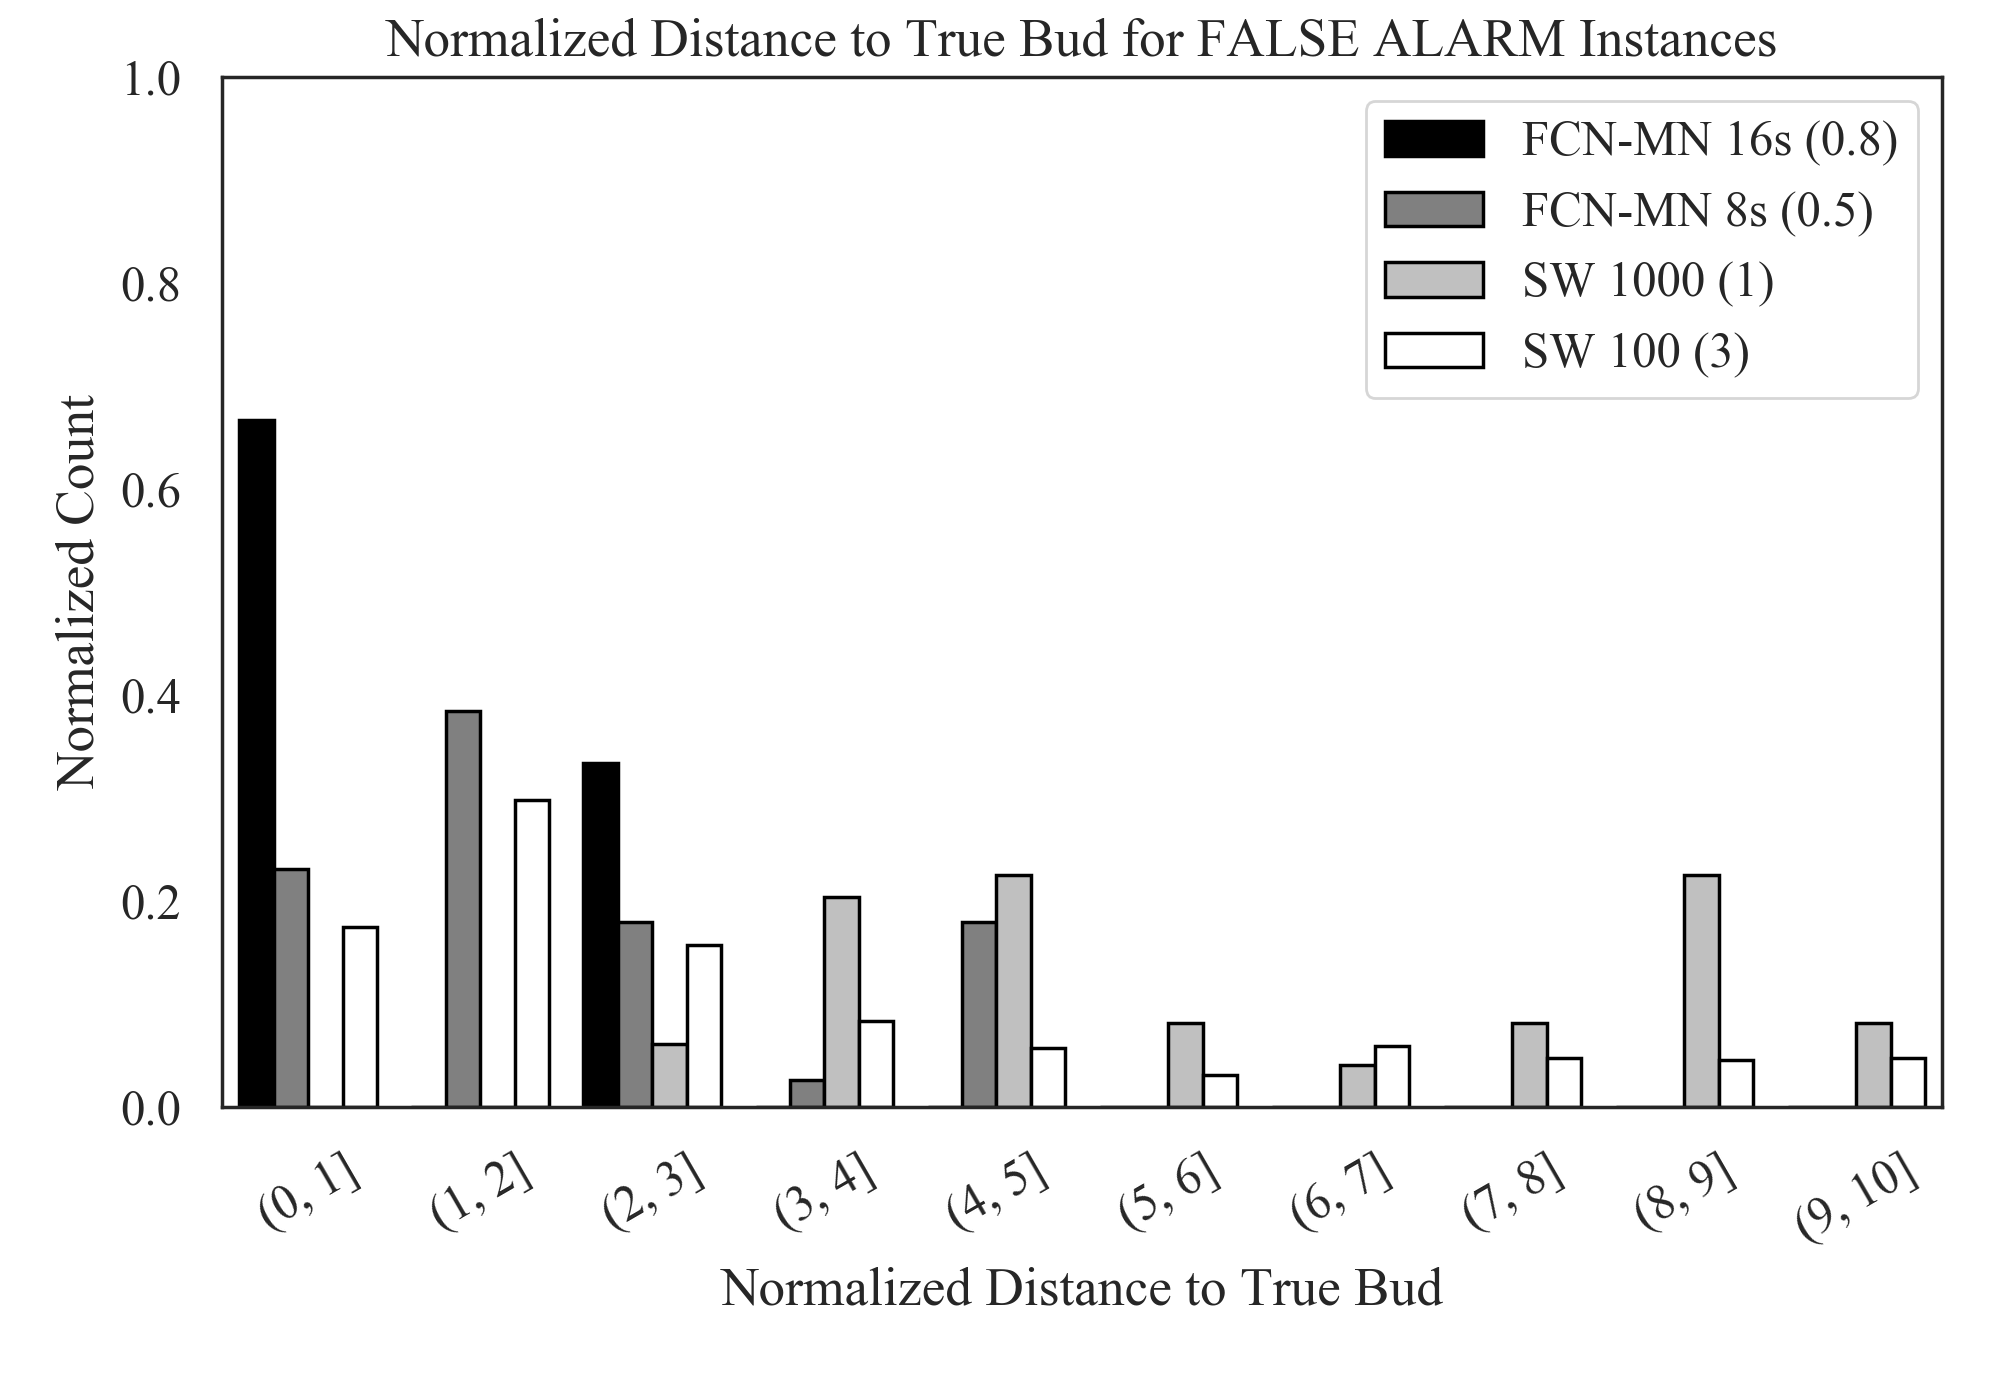
\includegraphics[width=\textwidth]{figures/CCC_normalized_distance_false_alarm.png}
		\caption{}
		\label{fig:CCC-b}
	\end{subfigure}
	\caption{Figure CCC  b for the normalzed distances (ND) .....}%
	\label{fig:CCC}%
\end{figure}

To further understand the results at a more refined level, we repeated the analysis performed for correct detections and splits, reporting the NA and ND over individual components for the same four models selected of higher mean F1 detection measure and the one with higher mean Dice metric for both FCN and SW. Again, we group them in histograms, shown in Figures \ref{fig:CCC-a} and \ref{fig:CCC-b} NA and ND, respectively. Here, the bars represent (normalized) counts of false alarm components. It is not a surprise that these figures confirm the improvements of FCN over SW reported for the mean over images (Figure \ref{fig:AAA}). For these four models in particular, they show that all false alarm components for FCN have an area smaller than that of the bud, i.e., an NA smaller than 1.0, whereas for SW we can observe false alarm components of sizes as large as $10$ time of that of the actual bud. Figure \ref{fig:CCC-b} shows, for these four models, that absolutely all false alarm components for the FCN case are within $2$ diameters of the true bud, whereas those of SW span to distances up to $10$ bud diameters. Interestingly, the distances for FCN are so small, that these false positive components could be easily interpreted as correct detections with a “relaxed” split, depending, of course, on the application for which these detections should be used.   One possible explanation for these nearby false alarms is that near the buds there is the knot, a part of the plant that even a naked eye could sometimes confuse with a bud. Under this relaxation of what we call correct detection, these two FCN models would present not a single false alarm, or equivalently, a perfect detection-precision.


%##############################################################
%##############################################################

\section{5. Discusión} \label{sec:discussion}

Presentación de la sección.
Enunciado del problema de medición autónoma de yemas (de forma resumida, NO copy\&paste de la intro) junto a la importancia de contar con una solución autónoma (¿cual? medición autónoma de variables vía la extracción autonoma de información geometríca, y visual segmentada para cada PoP).
Resumen del enfoque propuesto y del resultado principal (i.e. decir que mejora el estado del arte pero resumiendo en una o dos oraciones lo que SIN repetir lo que ya se dijo en el análisis de resultados), y argumento de la importancia de este resultado en el contexto de medición autónoma de yemas.
Presentación del caso concreto FCN-16s-0.5, argumentando por qué lo elegimos, junto al análisis y discusión de sus resultados:
Resumen de los resultados de detección (traer párrafo desde la sección Resultados Sistemáticos).
Resumen de los resultados de segmentación
Resumen de los resultados “detallados”, i.e. traer discusión y gráficos de subsecciones “Detailed analysis...” pero solo para el caso FCN-16s-0.5.
Discusión de estos resultados sobre las variables de la tabla 1 y como afecta a las sub-operaciones de detección 
Aquellas para las que el enfoque representa una solución directa:
conteo de yemas, que requiere individualización
bud area, que requiere segmentación + individualización
Aquellas que requieren soluciones adicionales
longitud de entre nudo, que requiere individualización + localización
Alguna otra?
Limitaciones generales del enfoque
Future works/directions

% =========================================================
% =========================================================


En esta sección se discuten los resultados obtenidos para la detección de yemas de vid y su impacto como una herramienta para la medición de variables vitícolas de interés. Para esto primero resulta útil revisar algunos aspectos de la medición manual de las variables asociadas a la yema (ver Tabla \ref{tab:Tabla1}), tal como se realiza en la práctica. 



Por otro lado, vamos a contrastar estos resultados con el método tradicional de conteo manual. En principio se podría pensar que el conteo manual comete pocos errores, alcanzando una detection-precision y una detection-recall de 1 (o al menos muy cercana). Sin embargo, el conteo manual de yemas tiene varias limitaciones que hacen imposible alcanzar estos valores: (i) no se realiza de forma exhaustiva sobre toda la planta, sino que se toma una muestra y se extrapola la cantidad total, con el correspondiente acarreo de errores durante la estimación; (ii) el proceso de medición manual en campo, en general, produce fatiga, por lo que es propenso a errores de conteo involuntarios; y (iii) es un proceso imposible de realizar sobre todas las plantas del campo, debido a la desmesurada cantidad de recursos que esto requeriría. 



se toman las variables de la Tabla 1 presentada en la introducción y se analiza individualmente el impacto de estos resultados para cada una de ellas.



El conteo de yemas es una variable que solo requiere de una tecnología de detección de yemas efectiva para poder realizar su medición de forma autónoma. Concretamente, contar yemas se requiere individualizar cada una de las yemas visibles en la escena (ver Table 1), por lo que las detection metrics resultan relevantes para analizar el impacto del enfoque FCN-MN (ver sección \ref{subsec:detectmetrics}). 
%
Tomando la información presentada en la Tabla \ref{tab:TablaXX} vamos a analizar los resultados de la FCN-MN con mayor F-measure. Este modelo alcanza una detection-precision de $0.977$ y un detection-recall de $0.921$, lo que significa que del total de detecciones de yema realizadas aproximadamente un $2\%$ son false alarm (i.e. errores por exceso en el conteo) y existe un $8\%$ de detection failure (i.e. errores por defecto en el conteo). 
%
Considerando que las plantas fotografiadas en promedio tienen
unas 240 yemas (esto depende de muchos factores, como ser sistema de conducción, varietal, tipo de tratamiento, época del año, entre otros), el enfoque propuesto contaría 5 yemas en exceso, y omitiría contabilizar 19 yemas. Si bien estos errores durante la detección producen un conteo erróneo de yemas, podrían mitigarse realizando un análisis que permita caracterizar estadísticamente ámbos errores. 
%
Como se mencionó anteriormente en la sección \ref{sub:compFCNSW}, algunos de los componentes detectados correctamente pueden ser splits. Ante una situación de split, si cada componente se contabiliza como una yema diferente entonces se introduce un error por exceso en el conteo final. Para el caso del modelo elegido, 

Por otro lado, vamos a contrastar estos resultados con el método tradicional de conteo manual. En principio se podría pensar que el conteo manual comete pocos errores, alcanzando una detection-precision y una detection-recall de 1 (o al menos muy cercana). Sin embargo, el conteo manual de yemas tiene varias limitaciones que hacen imposible alcanzar estos valores: (i) no se realiza de forma exhaustiva sobre toda la planta, sino que se toma una muestra y se extrapola la cantidad total, con el correspondiente acarreo de errores durante la estimación; (ii) el proceso de medición manual en campo, en general, produce fatiga, por lo que es propenso a errores de conteo involuntarios; y (iii) es un proceso imposible de realizar sobre todas las plantas del campo, debido a la desmesurada cantidad de recursos que esto requeriría. 

Tamaño de yema (área)


Finalmente, vale la pena destacar que el enfoque propuesto en este trabajo todavía presenta al menos tres limitaciones importantes para convertirse en una solución efectiva para la medición de variables asociadas a la detección de yemas: (i) la experimentación se realiza sobre un conjunto de imágenes con exactamente una yema cada una; (ii) si bien las imágenes fueron adquiridas en condiciones naturales de campo, la captura fue realizada por operarios que pueden haber influido involuntariamente en la construcción de un dataset sesgado según diferentes aspectos, como ser distancia a la yema, ángulo o vista, perspectiva, enfoque, entre otros; y (iii) no presenta ningún mecanismo para evitar el doble conteo de la misma yema en imágenes diferentes.

IDEA 1: revisar discusión del paper de detección de yemas 3D.

IDEA 2: agregar como impactaría el uso del nuevo clasificador en el enfoque de detección de yemas 3D

IDEA: discutir las posibilidades de medición de variables real time?

IDEA: decir algo respecto a uso de postprocesamientos durante la segmentación, como uso de features de forma o tamaños relativos


%·················································
\section{Conclusions} \label{sec:conclusion}

TODO: Conclusions

\section*{Acknowledgments}

Tal vez a alguien.

\section*{References}
\bibliography{2020-DeepBudDetection-CEA}

\end{document}